% Paquets généraux
\documentclass[a4paper,12pt,titlepage,twoside]{article}
\usepackage[T1]{fontenc}
\usepackage[utf8]{inputenc}
\usepackage[french]{babel}
\usepackage{subcaption}
\addto\captionsfrench{%
  \renewcommand{\tablename}{Tableau}%
}
\usepackage[gen]{eurosym}
%\usepackage[dvips]{graphicx}
\usepackage{minted}
\usepackage{fancyhdr}
\usepackage{pdfpages} 
\usepackage{multido}
\usepackage{hyperref}
\usepackage{textcomp}
\usepackage{schemabloc}
%\usepackage[bitstream-charter]{mathdesign}
\usepackage{array}
\newcolumntype{P}[1]{>{\centering\arraybackslash}p{#1}}
\usepackage[shortlabels]{enumitem}
\usepackage[framemethod=TikZ]{mdframed}

\newcommand{\id}{71}
\newcommand{\nom}{Théorie des mécanismes}
\newcommand{\sequence}{04}
\newcommand{\nomsequence}{Liaisons entre les solides}
\newcommand{\num}{02}
\newcommand{\type}{KH}
\newcommand{\descrip}{Liaisons équivalentes, hyperstatisme, liaisons en série et en parallèle, théorie des graphes}
\newcommand{\competences}{B2-12: Proposer une modélisation des liaisons avec leurs caractéristiques géométriques. \\ &  B2-13: Proposer un modèle cinématique paramétré à partir d'un système réel, d'une maquette numérique ou d'u \\ &  B2-17: Simplifier un modèle de mécanisme. \\ &  B2-18: Modifier un modèle pour le rendre isostatique. \\ &  C1-04: Proposer une démarche permettant d'obtenir une loi entrée-sortie géométrique.  \\ &  C2-05: Caractériser le mouvement d'un repère par rapport à un autre repère. \\ &  C2-06: Déterminer les relations entre les grandeurs géométriques ou cinématiques. }
\newcommand{\nbcomp}{7}
\newcommand{\systemes}{}
\newcommand{\systemesnum}{}
\newcommand{\systemessansaccent}{}
\newcommand{\ilot}{2}
\newcommand{\ilotstr}{02}
\newcommand{\dossierilot}{\detokenize{Ilot_02 }}

%\usepackage{style}
\usepackage{bodegraph}
\usepackage{rpcinematik}
\usepackage[locale = FR]{siunitx}
\usepackage{caption}
\newcommand{\institute}{Lycée Dorian}

\usepackage{listings}
\usepackage{fancyvrb}
\usepackage{color}
\usepackage{xcolor}
\usepackage{colortbl}
\usepackage{helvet}
\usepackage[frenchmath]{newtxsf} % for sans serif symbols
\renewcommand{\familydefault}{\sfdefault}
%\usepackage{amsfonts}
%\usepackage{amsmath}
%\usepackage{lmodern}
\usepackage{mathastext}
%\usepackage{xspace}
\usepackage{varioref}
\usepackage{tabularx}
%\usepackage{floatflt}
\usepackage{graphics}
\usepackage{wrapfig}
\usepackage{textcomp}
\usepackage{tikz,tkz-tab}
\usepackage[european resistor, european voltage, european current]{circuitikz}
\usepackage{wrapfig}
\usepackage{gensymb}
\usepackage[percent]{overpic}
\usetikzlibrary{babel}
\usepackage{ifthen}
\usepackage{cancel}
\usepackage{etoolbox}
\usepackage{multirow}
%\usepackage{boxedminipage}
\definecolor{gris25}{gray}{0.75}
\definecolor{bleu}{RGB}{18,33,98}
\definecolor{bleuf}{RGB}{42,94,171}
\definecolor{bleuc}{RGB}{231,239,247}
\definecolor{bleum}{RGB}{160,195,226}
\definecolor{rougef}{RGB}{185,18,27}
\definecolor{rougec}{RGB}{255,188,204}%255,230,231
\definecolor{vertf}{RGB}{103,126,82}
\definecolor{vertc}{RGB}{220,255,191}
\definecolor{forestgreen}{rgb}{0.13,0.54,0.13}
\definecolor{blcr}{rgb}{0.59,0.69,0.84}
\definecolor{blfr}{rgb}{0.32,0.51,0.75}
\definecolor{orfr}{rgb}{0.90,0.42,0.15}
\definecolor{orcr}{rgb}{0.90,0.65,0.50}
\definecolor{orangef}{rgb}{0.659,0.269,0.072}
\definecolor{orange}{rgb}{0.58,0.35,0.063}
\definecolor{orangec}{rgb}{0.43,0.32,0.25}
\definecolor{rcorrect}{rgb}{0.6,0,0}
\definecolor{sequence}{rgb}{0.75,0.75,0.75}
\definecolor{competences}{rgb}{0.61,0.73,0.35}
\definecolor{rose}{HTML}{ff00ff}
\definecolor{grisf}{HTML}{222222}
\definecolor{grisc}{HTML}{636363}
\definecolor{normal}{HTML}{4087c4}
\definecolor{info}{HTML}{5bc0de}
\definecolor{success}{RGB}{92,184,92}
\definecolor{warning}{RGB}{240,173,78}
\definecolor{danger}{RGB}{217,83,79}
\hypersetup{                    % parametrage des hyperliens
    colorlinks=true,                % colorise les liens
    breaklinks=true,                % permet les retours à la ligne pour les liens trop longs
    urlcolor= blfr,                 % couleur des hyperliens
    linkcolor= orange,                % couleur des liens internes aux documents (index, figures, tableaux, equations,...)
    citecolor= forestgreen                % couleur des liens vers les references bibliographiques
    }

\newcolumntype{M}[1]{>{\centering\arraybackslash}m{#1}}
\definecolor{codegreen}{rgb}{0,0.6,0}
\definecolor{codegray}{rgb}{0.5,0.5,0.5}
\definecolor{codepurple}{rgb}{0.58,0,0.82}
\definecolor{backcolour}{rgb}{0.95,0.95,0.92}

\lstdefinestyle{mystyle}{
    backgroundcolor=\color{backcolour},   
    commentstyle=\color{codegreen},
    keywordstyle=\color{magenta},
    numberstyle=\tiny\color{codegray},
    stringstyle=\color{codepurple},
    basicstyle=\ttfamily\footnotesize,
    breakatwhitespace=false,         
    breaklines=true,                 
    captionpos=b,                    
    keepspaces=true,                 
    numbers=left,                    
    numbersep=5pt,                  
    showspaces=false,                
    showstringspaces=false,
    showtabs=false,                  
    tabsize=2
}

\lstset{style=mystyle}

% Mise en page
\pagestyle{fancy}

\setlength{\hoffset}{-18pt}
\setlength{\oddsidemargin}{0pt} 	% Marge gauche sur pages impaire2s
\setlength{\evensidemargin}{0pt} 	% Marge gauche sur pages paires
\setlength{\marginparwidth}{00pt} 	% Largeur de note dans la marge
\setlength{\headwidth}{481pt} 	 	% Largeur de la zone de tête (17cm)
\setlength{\textwidth}{481pt} 	 	% Largeu\textbf{r de la zone de texte (17cm)
\setlength{\voffset}{-18pt} 		% Bon pour DOS
\setlength{\marginparsep}{7pt}	 	% Séparation de la marge
\setlength{\topmargin}{-30pt} 		% Pas de marge en haut
\setlength{\headheight}{55pt} 		% Haut de page
\setlength{\headsep}{20pt} 		% Entre le haut de page et le texte
\setlength{\footskip}{30pt} 		% Bas de\textbf{ page + séparation
\setlength{\textheight}{700pt} 		% Hauteur de l'icone zone de texte (25cm)
\setlength\fboxrule{1 pt}
\renewcommand{\baselinestretch}{1}
\setcounter{tocdepth}{1}
\newcommand{\cadre}[2]
{\fbox{
  \begin{minipage}{#1\linewidth}
   \begin{center}
    #2\\
   \end{center}
  \end{minipage}
 }
}

\newcommand{\repon}[1]
{
~\ \\
\begin{tabular}{|m{\linewidth}|}
 \hline
\multido{}{#1}{\\ \hline}
\end{tabular}
}


\newcommand{\objectif}[1]{
\mdfsetup{%
frametitle={%
\tikz[baseline=(current bounding box.east),outer sep=0pt]
\node[anchor=east,rectangle,fill=bleum]
{\strut Objectif~};}}
\mdfsetup{innertopmargin=10pt,linecolor=bleum,%
linewidth=2pt,topline=true,%
frametitleaboveskip=\dimexpr-\ht\strutbox\relax
}
\begin{mdframed}[]\relax%
#1
\end{mdframed}}


\newcounter{num_quest} \setcounter{num_quest}{0}
\newcounter{num_rep} \setcounter{num_rep}{0}
\newcounter{num_cor} \setcounter{num_cor}{0}

\newcommand{\feuilleDR}[1]{
	\begin{tikzpicture}
		\draw[gray!30](0,0)grid[step=0.5cm](\linewidth,#1);
	\end{tikzpicture}
}

%\newcommand{\question}[1]{\refstepcounter{num_quest}\par
%~\ \\ \parbox[t][][t]{0.15\linewidth}{\textbf{Question \arabic{num_quest}}}\parbox[t][][t]{0.85\linewidth}{#1\label{q\the\value{num_quest}}}\par
%}

\newcommand{\question}[1]{\refstepcounter{num_quest}\par
~\ \\ \textbf{Question \arabic{num_quest} : }#1\label{q\the\value{num_quest}}\par
}

\newcommand{\posetafigure}[3]{
\begin{figure}[ht!]
 \begin{center}
  \includegraphics[width=#2\linewidth]{img/#1}
 \end{center}
 \caption{\label{#1} #3}
\end{figure}}

\newcommand{\goforum}{
\begin{figure}

\end{figure}
\begin{center}
 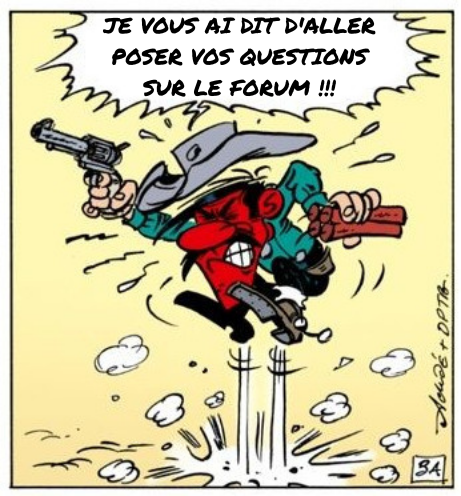
\includegraphics[width=0.7\linewidth]{../../../img/go_forum}
\end{center}
\label{go_forum}
\caption{J'pète les plombs}
\end{figure}}

\newcommand{\reponse}[4][1]
{\noindent
\parbox{\textwidth}{
\rule{\linewidth}{.5pt}\\
\textbf{Question\ifthenelse{#1>1}{s}{} \multido{}{#1}{%
\refstepcounter{num_rep}\ref{q\the\value{num_rep}} }:} ~\ \\
\ifdef{\public}{#3 \ifthenelse{#2>0}{~\ \\ 	\feuilleDR{#2}}}{#4}
}}

\newcommand{\cor}
{\refstepcounter{num_cor}
\noindent
\rule{\linewidth}{.5pt}
\textbf{Question \arabic{num_cor}:} \\
}

\newcommand{\finsujet}
{
    \begin{center}
    \Large{FIN}
    \end{center}

    \cleardoublepage

    \ifdef{\public}{\pagestyle{docreponse}}{\pagestyle{correction}}

    \ifdef{\public}{
        \begin{tikzpicture} 
            \draw (0,0) rectangle (2,2);
            \draw (0,0) -- (2,2);
            \draw (1.5,0.5) node {\large 20};
            \draw (2.5,0) rectangle (16,2);
            \draw (4.5,1.7) node {\large Commentaires:};
        \end{tikzpicture}
    }
    ~\ \\
}


%\newcommand{\repcarre}[2]
%{
%~\ \\
%\begin{tikzpicture}
%\draw [fill=white] (0,0) rectangle +(\linewidth,#1);
%\node[align=left] at (1.1,#2-0.3) {\textbf{Question #1:}};
%\end{tikzpicture}
%}

\newcommand{\titre}[1]
{\begin{center}
\cadre{0.8}{\huge #1} 
\end{center}
}


%Définition des torseurs :
\newcommand{\torseur}[2]{\left\{\mathcal{#1}_{#2} \right\}}
\newcommand{\torseurh}[3]{\left\{\genfrac{}{}{0pt}{0}{#1}{#2}\right\}_{#3}}
\newcommand{\torseurv}[8]{\left\{
\begin{matrix}
#1 & #4 \\ #2 & #5 \\ #3 &#6
\end{matrix}
\right\}_{{#7},{#8}}}

%Définition des torseurs :
%\newcommand{\torseur}[2]{\left \{\mbox{\relsize{2}{$\mathcal {#1}$}\relsize{-2}}\phantom{}_{\mbox{\scriptsize $#2$}} \right \}}
%\newcommand{\torseurh}[3]{\left\{\genfrac{}{}{0pt}{0}{#1}{#2}\right\}_{#3}}
%\newcommand{\torseurv}[8]{
%\left\{\begin{array}{@{}c|c@{}} #1 & #4 \\ #2 & #5 \\ #3 & #6 \end{array} \right\}_{#7,#8}
%}
\newcommand{\derivee}[2]{\left.\dfrac{\d #1}{\d t}\right|_{#2}}
\newcommand{\tripleint}{\int\!\!\!\!\!\int\!\!\!\!\!\int}

% Notation cinématique et statique
\newcommand{\cinematique}[2]{\mbox{#1}/\mbox{#2}}
\newcommand{\statique}[2]{\mbox{#1}\rightarrow\mbox{#2}}
\newcommand{\moment}[3]{\vv {#1}_{\scriptsize{#3}}(#2)}
\newcommand{\resultante}[2]{\vv {#1}_{\scriptsize{#2}}}


%Commande de base
\newcommand{\jo}{\left(j\omega\right)} % j \omega dans l'analyse fréquentielle
\newcommand{\tl}{\xrightarrow{\mathcal{L}}} % transformée de laplace sur fleche
\newcommand{\tli}{\xrightarrow{\mathcal{L}^{-1}}} % transformée inverse de laplace sur fleche
\renewcommand{\d}[1][]{\mathrm{d#1}}
\newcommand{\dd}[1][]{\mathrm{d#1}}
\newcommand{\vect}[2]{{#1}\wedge{#2}}
\newcommand{\base}[3]{(\vec #1,\vec #2,\vec #3)}
\newcommand{\vectbase}[4]{{\vphantom{\left| \begin{matrix}
#1\\#2\\#3 \end{matrix} \right|}}_{#4}{\left| \begin{matrix}
#1\\#2\\#3 \end{matrix} \right.}}
%Pour avoir les paragraphes sous la forme I, II, III
\renewcommand{\thesection}{\Roman{section}}
\setcounter{secnumdepth}{3}
\renewcommand{\Frlabelitemii}{$\bullet$}

% En tête et pied de page
\lhead{\nom}
\rhead{
\includegraphics[width=2cm]{../../../img/logo}}
\lfoot{\auteurun,\ \auteurdeux}
\cfoot{Page \thepage}

\fancypagestyle{docreponse}{%
  \fancyhf{}
  \fancyhead[LO]{NOM Prénom: .............................}
  \rhead{
\includegraphics[width=2cm]{../../../img/logo}\hspace{2pt}}
  \ifdef{\auteurdeux}{\lfoot{\auteurun,\ \auteurdeux}}{\lfoot{\auteurun}}
  \rfoot{\nom}
  \lfoot{Document réponse}
  \cfoot{Page \thepage}
   }

\fancypagestyle{correction}{%
  \fancyhf{}
  \lhead{\colorbox{danger}{\begin{minipage}{0.65\paperwidth} \textcolor{white}{\textbf{Correction}} \end{minipage}} }
  \rhead{
\includegraphics[width=2cm]{../../../img/logo}}
  \lfoot{Renaud Costadoat, Françoise Puig}
  \rfoot{\colorbox{danger}{\begin{minipage}{0.4\paperwidth} \begin{flushright}\textcolor{white}{\textbf{Correction}}\end{flushright} \end{minipage}} }}

\fancypagestyle{correctioninfo}{%
  \fancyhf{}
  \lhead{\colorbox{danger}{\begin{minipage}{0.65\paperwidth} \textcolor{white}{\textbf{Correction}} \end{minipage}} }
  \rhead{
\includegraphics[width=2cm]{../../../img/logo}}
  \lfoot{Renaud Costadoat, Juliette Genzmer}
  \rfoot{\colorbox{danger}{\begin{minipage}{0.6\paperwidth} \begin{flushright}\textcolor{white}{\textbf{Correction}}\end{flushright} \end{minipage}} }}

\renewcommand{\footrulewidth}{0.4pt}

\usepackage{eso-pic}
\newcommand{\BackgroundPic}{%
\put(0,0){%
\parbox[b][\paperheight]{\paperwidth}{%
\vfill
\begin{center}
\hspace{0.5cm}\vspace{0.5cm}
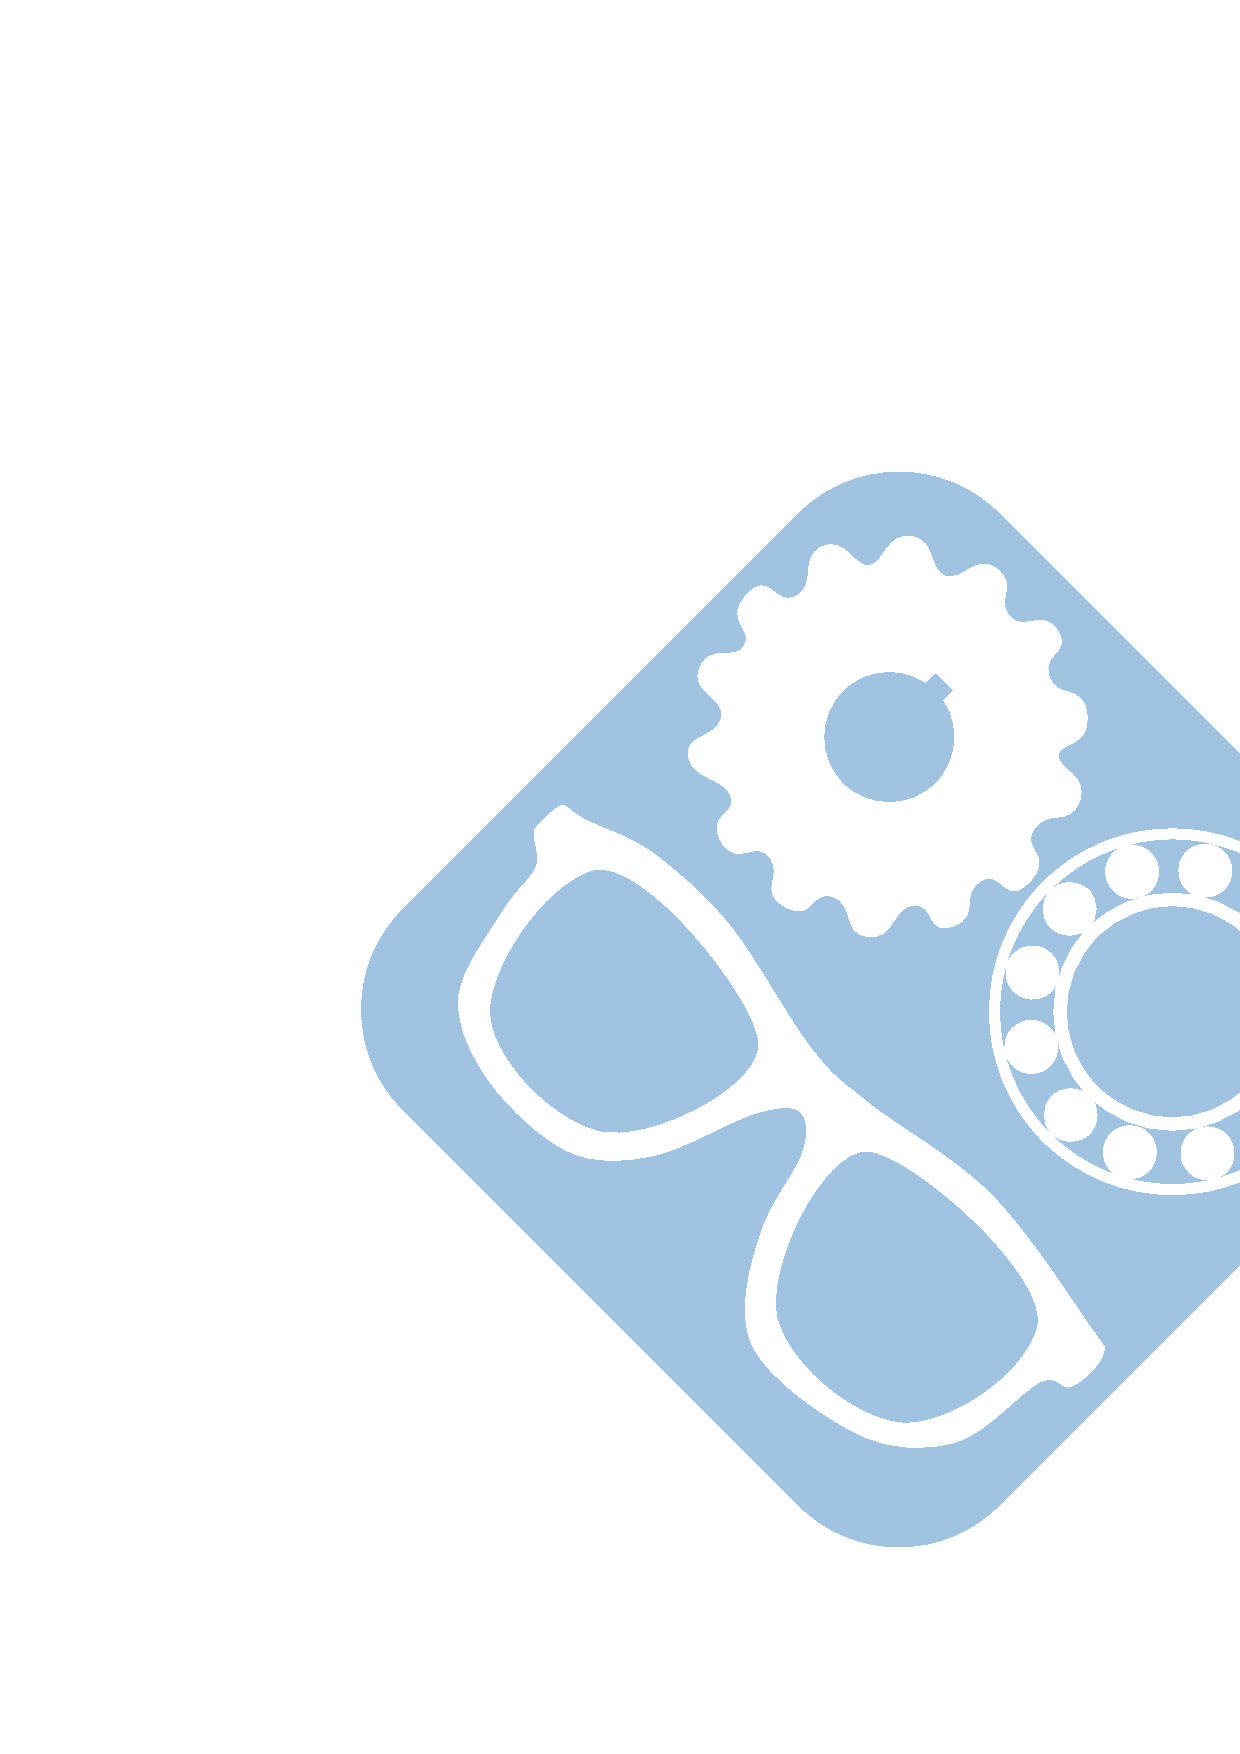
\includegraphics[width=\paperwidth,height=\paperheight,%
keepaspectratio]{../../../img/fond3}%
\end{center}
\vfill
}}}

\newcommand{\BackgroundPicdeux}{%
\put(25,-30){%
\parbox[b][\paperheight]{\paperwidth}{%
\vfill
\begin{center}
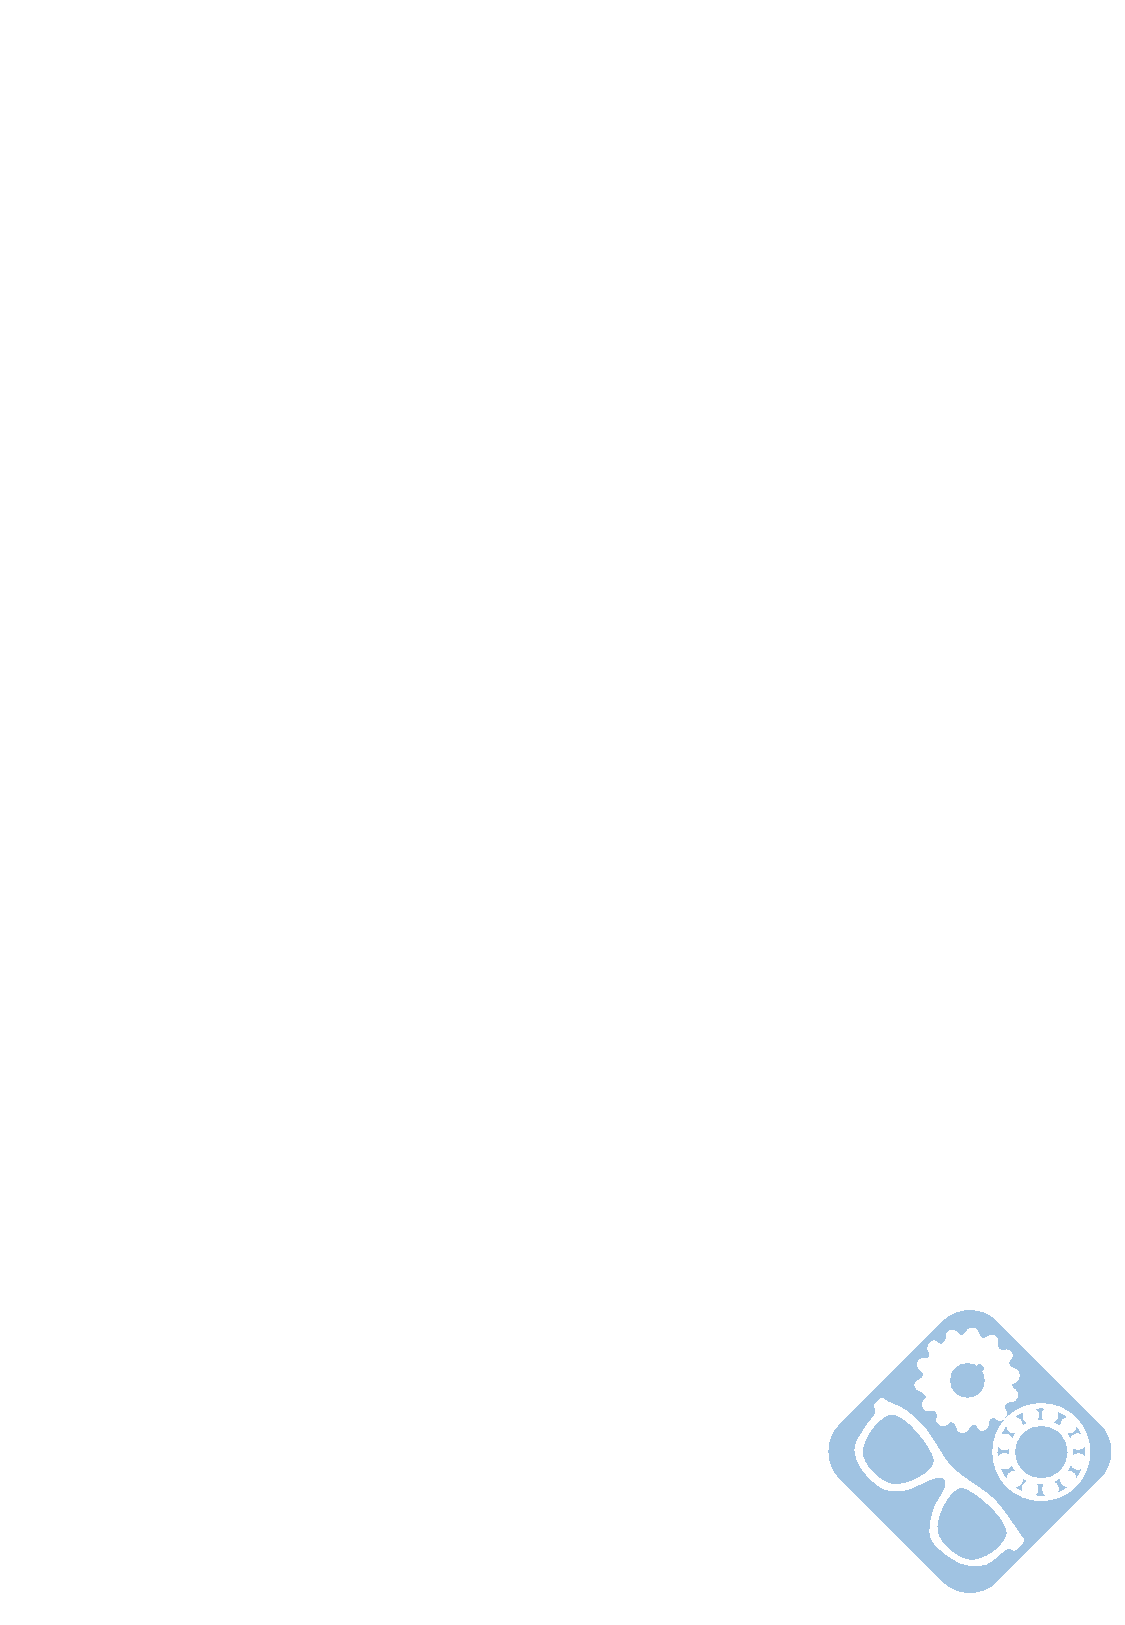
\includegraphics[width=\paperwidth,height=\paperheight,%
keepaspectratio]{../../../img/fond4}%
\end{center}
\vfill
}}}

\begin{document}

\pagestyle{empty}

\AddToShipoutPicture*{\BackgroundPic}


\includegraphics[width=2cm]{../../../img/logo}

\Huge{DS \numero - \sujet}

\vspace{1cm}

\ifdef{\prive}{\begin{center}\colorbox{danger}{\Huge{Avec Correction}}\end{center}}{}

\begin{center}
\centering\huge{PTSI}
\end{center}

\vspace{2cm}


\begin{center}
\centering\Large{\jour}
\end{center}

\vspace{2cm}

\normalsize

\tableofcontents

\newpage

\AddToShipoutPicture{\BackgroundPicdeux}

\pagestyle{fancy}

\begin{center}
\Huge \sujet
\end{center}


\normalsize


\section{Mise en situation}

\subsection{Le contexte}

L'industrie manufacturière mobilise de nombreux procédés d'obtention de pièces qui composent
la plupart des produits utilisés par le monde. L'un de ces procédés, la découpe mécanique sous
presse, permet de découper des pièces métalliques avec un contour défini, figure \ref{fig01}, à partir
d'une bobine de tôle, figure \ref{fig02}.

\begin{figure}[!h]
\begin{minipage}{0.45\linewidth}
 \centering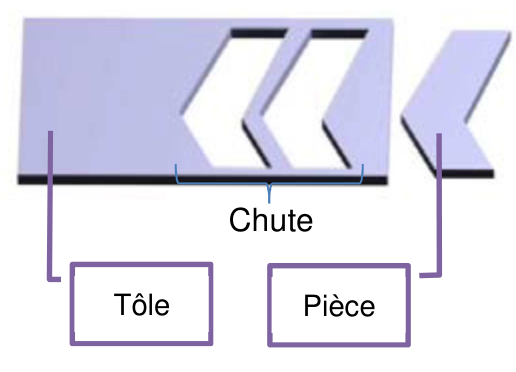
\includegraphics[width=0.7\linewidth]{img/fig1}
 \caption{Principe de découpe de pièces sous presse}
 \label{fig01}
\end{minipage}\hfill
\begin{minipage}{0.45\linewidth}
 \centering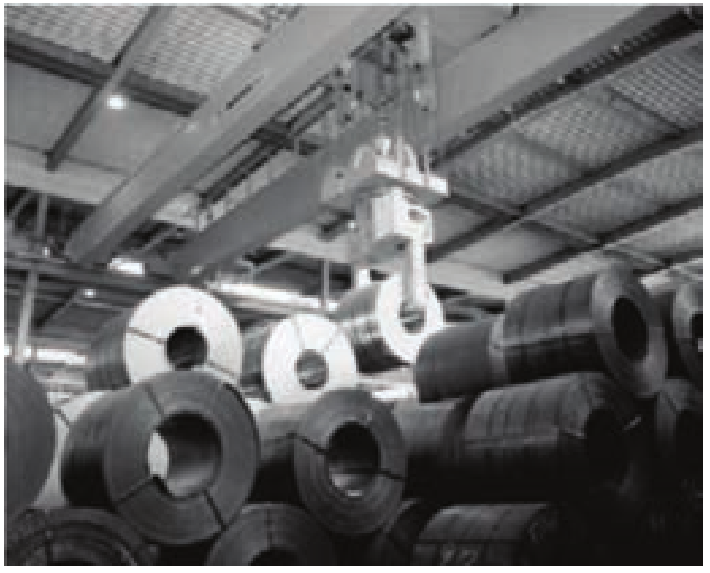
\includegraphics[width=0.7\linewidth]{img/fig2}
 \caption{Bobines de tôles métalliques}
 \label{fig02}
\end{minipage}
\end{figure}

L'opération de découpe est réalisée par une presse mécanique dont les principaux éléments de
la partie opérative sont un poinçon et une matrice dont les formes correspondent au contour de
la pièce à découper. La matrice est fixe, le poinçon a un mouvement de translation alternative
vertical. A chaque aller-retour du poinçon, une pièce est découpée dans la tôle. Pendant que le
poinçon est en position haute, la bande de tôle est déplacée horizontalement, figure \ref{fig03}.

\begin{figure}[!h]
 \centering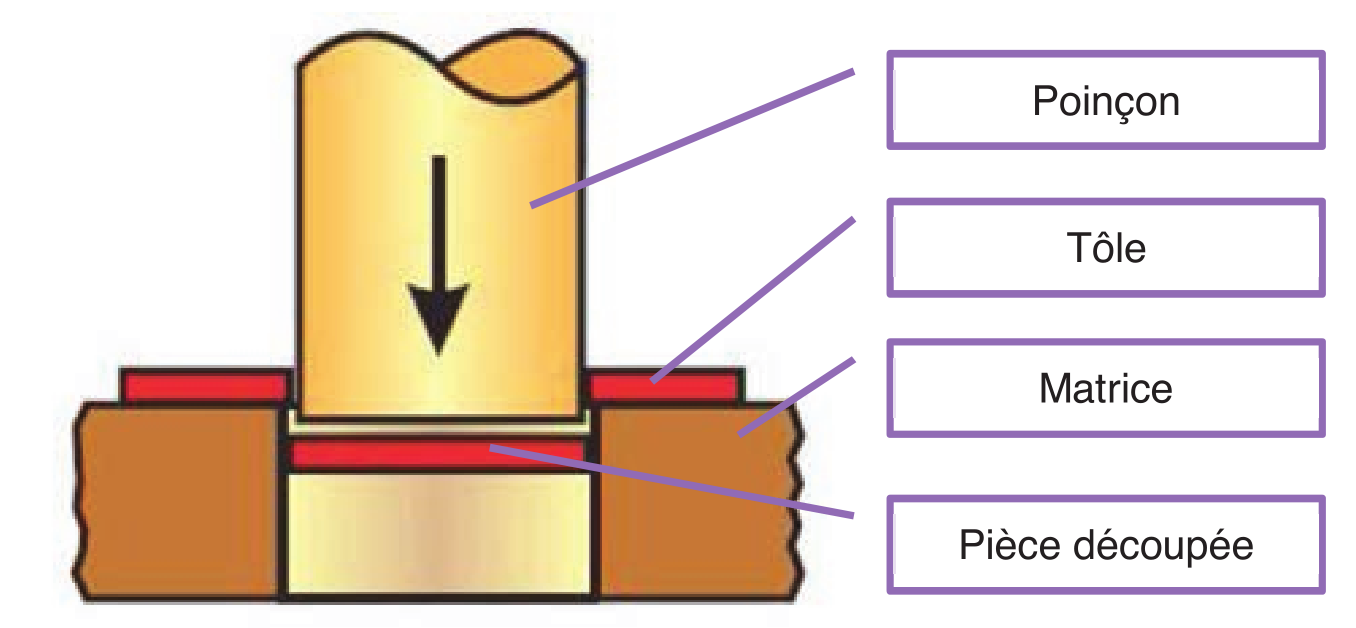
\includegraphics[width=0.7\linewidth]{img/fig3}
 \caption{Principe du poinçonnage}
 \label{fig03}
\end{figure}

\newpage

\subsection{Architecture d'une ligne de découpage}

Afin d'obtenir des cadences de production les plus élevées possible, la plupart des lignes de
découpe ont un niveau d'automatisation élevé. Ces lignes sont constituées généralement des
composants suivants, figure \ref{fig04}
\begin{itemize}
 \item un dérouleur : il supporte la bobine de tôle et déroule la bande à une vitesse continue,
 \item un redresseur : il corrige le défaut de planéité de la bande due à son enroulement,
 \item un dispositif d'amenage : il génère un mouvement de translation discontinu de la bande. En
effet, celle-ci qui doit être immobile pendant la phase de découpe, et se déplacer pendant le
moment ou le poinçon est dégagé de la matrice. Ce dispositif est synchronisé avec le
mouvement du poinçon,
 \item la presse : elle poinçonne la bande,
 \item une cisaille coupe-déchet : elle coupe les chutes de tôle pour en créer des déchets à
évacuer,
 \item un dispositif d'évacuation des pièces : il dirige les pièces réalisées vers la suite du
processus (contrôle, finition, montage,...),
 \item des dispositifs de contrôle : ils permettent de gérer les différences de vitesses de la bande
en agissant sur la taille des boucles de bande détendue et soumise à son poids propre.
\end{itemize}

\begin{figure}[!h]
 \centering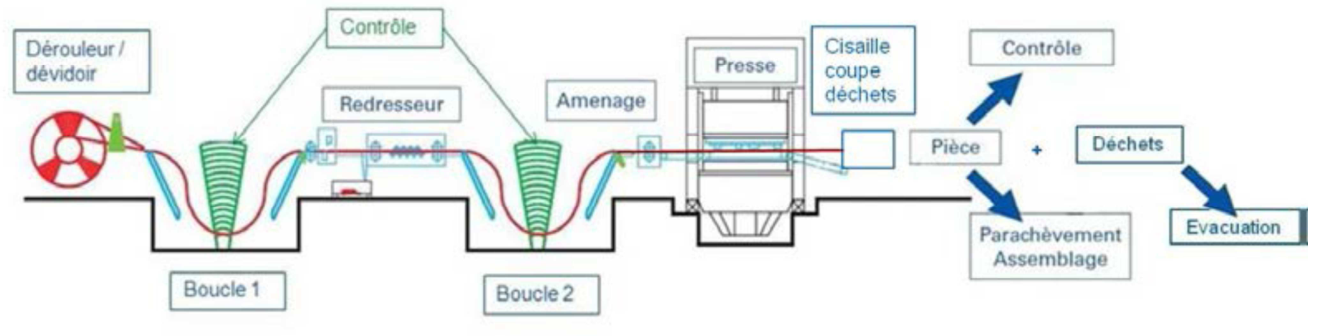
\includegraphics[width=0.7\linewidth]{img/fig4}
 \caption{Architecture standard d'une ligne de découpe automatisée}
 \label{fig04}
\end{figure}

\subsection{Le produit à concevoir}

L'étude qui vous est confiée est limitée au dérouleur de la ligne de découpage.

Une première étude a été menée. Elle a débouché sur un prototype qui a été testé et sur lequel différents
dysfonctionnements ont été constatés. Il vous appartient d'analyser le fonctionnement de certaines parties du
dérouleur, et d'en proposer des modifications dans l'objectif d'une fabrication en moyenne série.

\begin{figure}[!h]
 \centering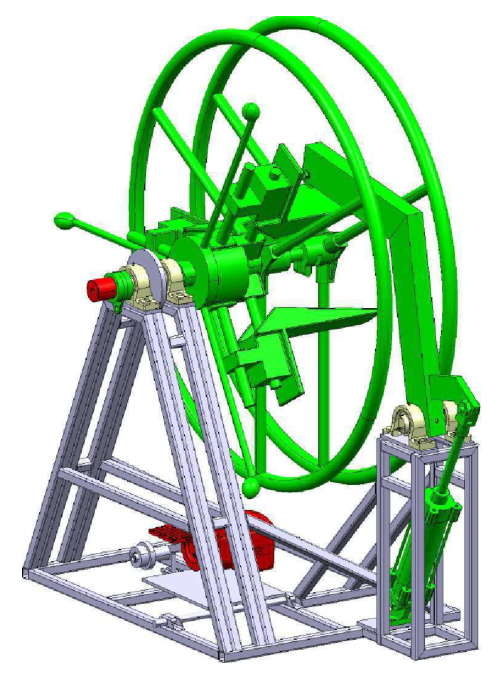
\includegraphics[width=0.2\linewidth]{img/fig5}
 \caption{Prototype de dérouleur}
 \label{fig05}
\end{figure}

\subsection{Diagramme des exigences}

Les principales exigences du dérouleur en phase de fonctionnement sont modélisées ci-dessous, figure \ref{fig06}.

\begin{figure}[!h]
 \centering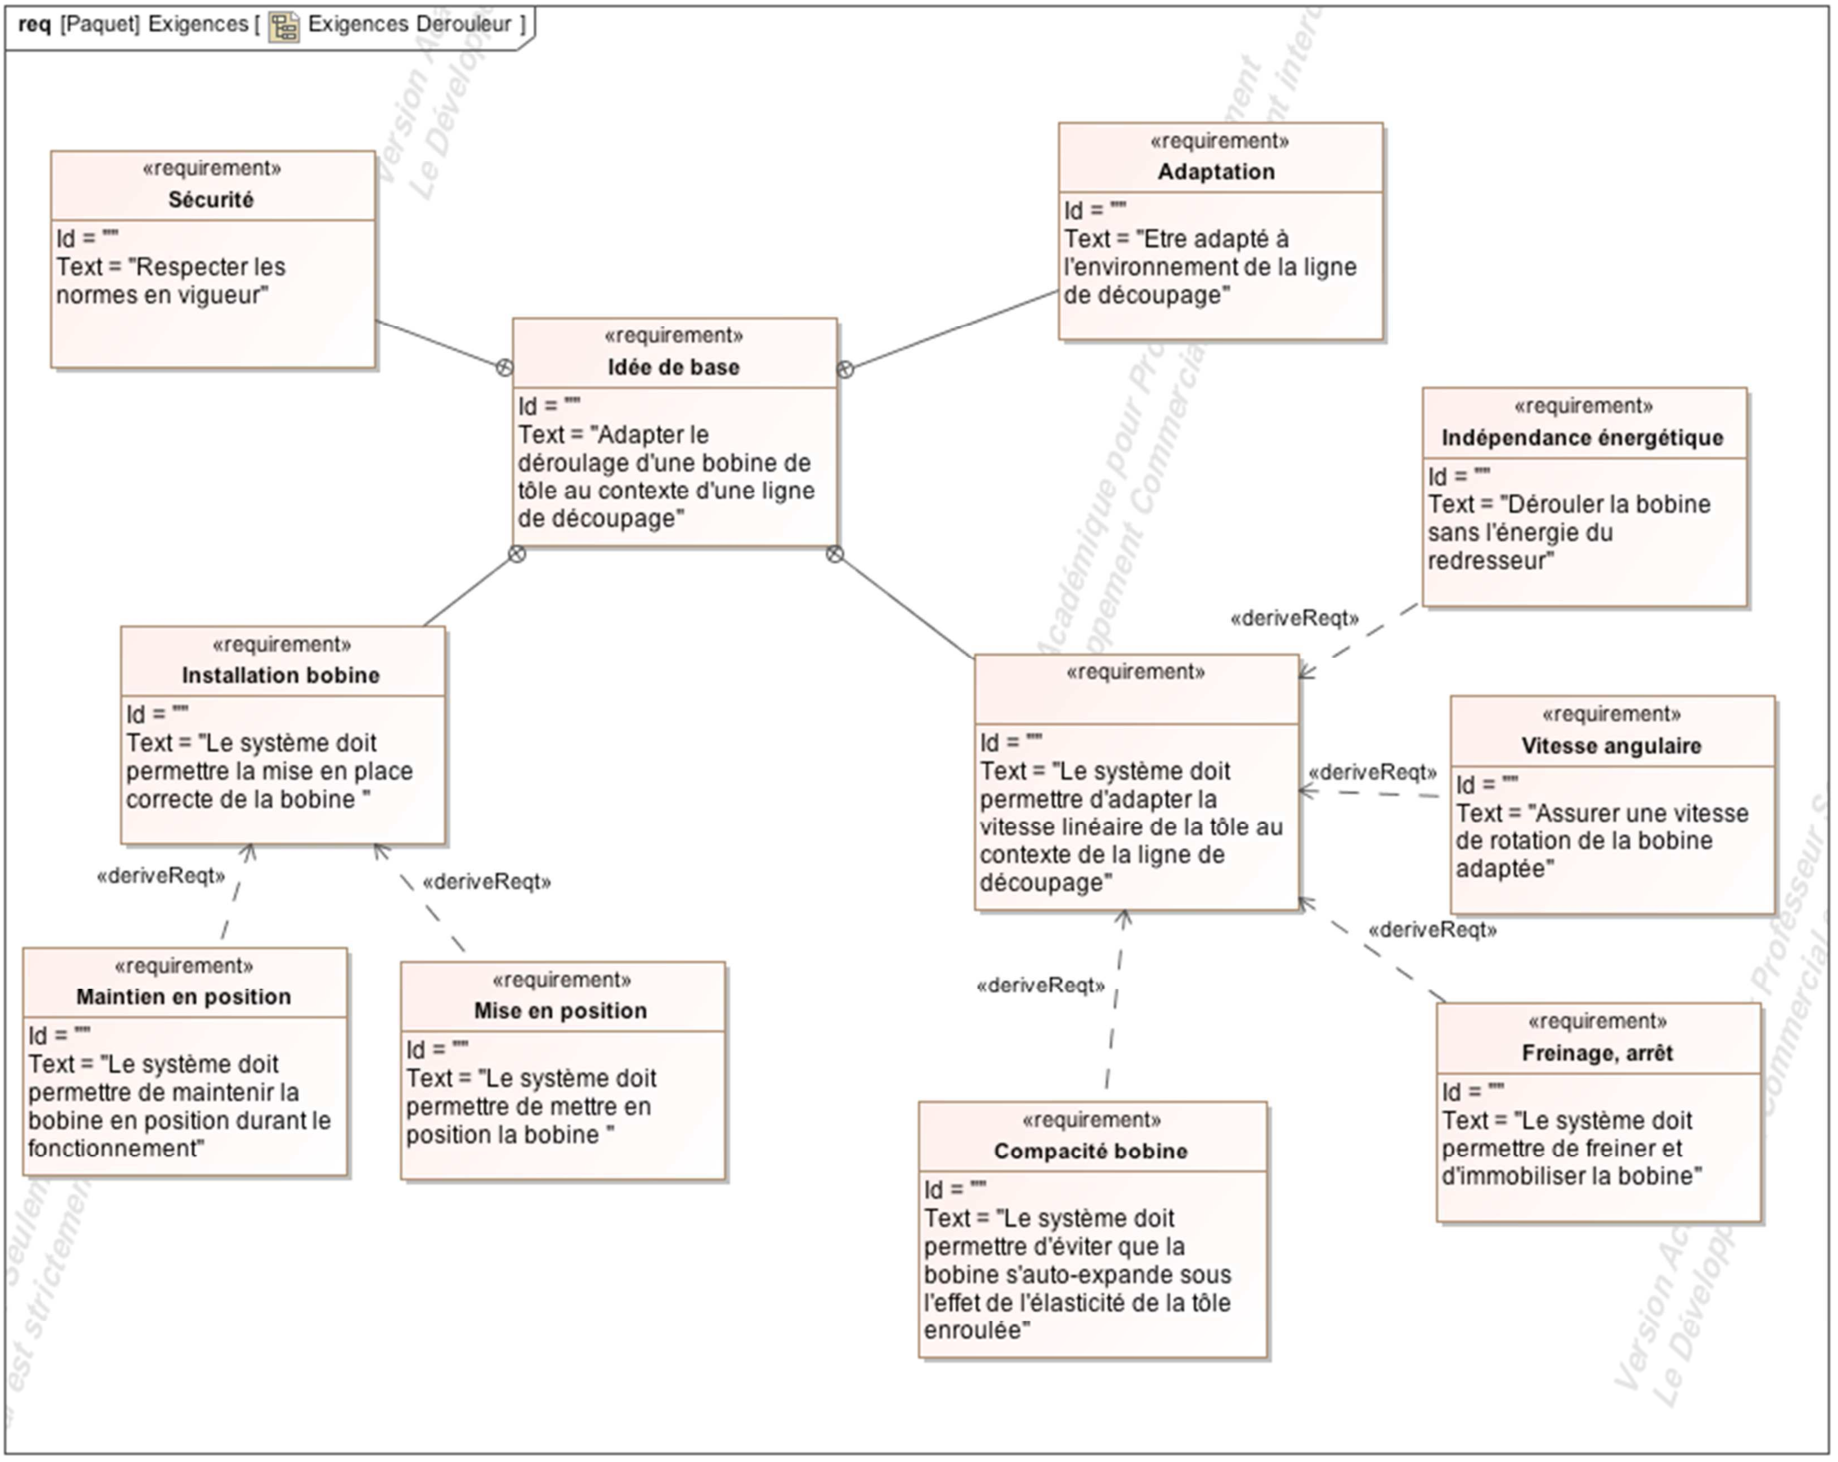
\includegraphics[width=0.7\linewidth]{img/fig6}
 \caption{Diagramme des exigences du dérouleur}
 \label{fig06}
\end{figure}

\section{Études et éléments de solutions proposés}

\subsection{Architecture du dérouleur}

L'architecture interne du dérouleur et le lien avec la ligne de découpage est décrite figure \ref{fig07}.

\begin{figure}[!h]
 \centering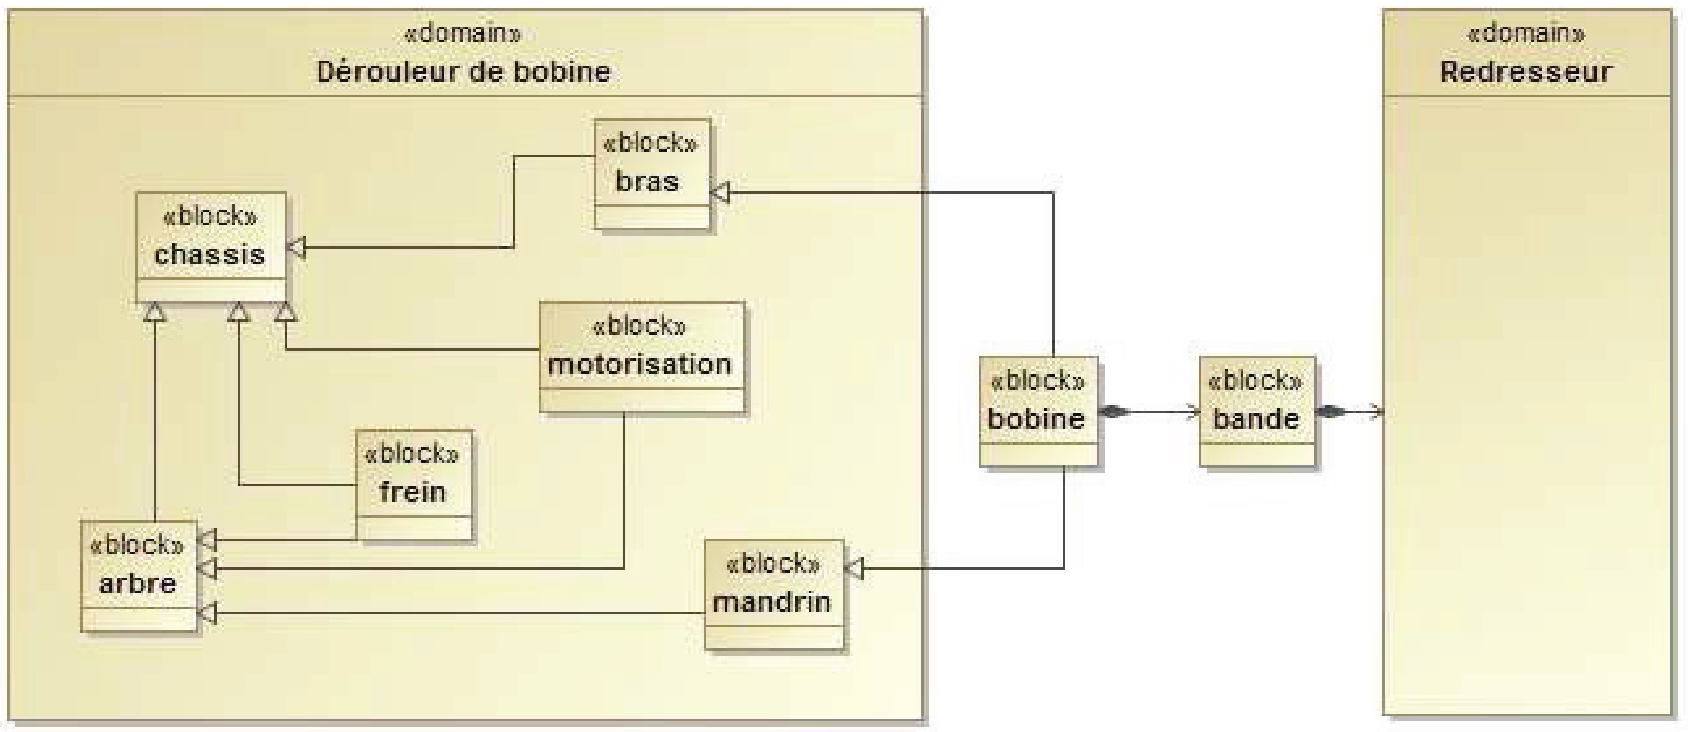
\includegraphics[width=0.7\linewidth]{img/fig7}
 \caption{Architecture interne du dérouleur}
 \label{fig07}
\end{figure}

\subsection{Problématique}

Dans la phase de re-conception il va falloir mener des études permettant l'amélioration du
fonctionnement du prototype du dérouleur. Il s'agit notamment de :
\begin{itemize}
 \item identifier les différents types de ligne de découpage influençant le fonctionnement du
dérouleur,
 \item re-concevoir le bras garantissant l'exigence \og anti retour élastique \fg,
 \item étudier le mandrin assurant les exigences \og mise en position \fg et \og maintien en
position \fg de la bobine de tôle par rapport au dérouleur,
 \item  étudier et implanter un nouveau frein réalisant l'exigence \og blocage \fg de la bobine.
Ces différentes études constituent la trame du travail à fournir dans ce sujet.
\end{itemize}

\section{Etude de conception en construction mécanique}

\subsection{Les différents types d'architecture de ligne de découpe}

Il existe différents types d'architecture pour une ligne de découpe. Le principal problème est de
gérer l'avancement discontinu de la tôle au niveau de la presse. En effet, lorsque la cadence de
production augmente, les accélérations au niveau de la bobine de tôle engendrent des efforts
importants.

Il existe donc différentes architectures de ligne de découpe, chacune adaptée à une cadence,
une dimension de bobine, une tâche à réaliser...

\paragraph{Objectif :} ~\ \\
L'inertie et l'énergie cinétique de la bobine de tôle peuvent poser des problèmes pour réaliser
une alimentation discontinue du système, surtout si les cadences sont élevées. C'est pourquoi,
il existe (ou non) des \og boucles \fg de tôle dans la chaîne d'alimentation de la presse, afin d'avoir
un déroulement à vitesse régulée de la bobine avec une variation progressive de la fréquence
de rotation, alors que la presse est alimentée de manière discontinue.

\begin{figure}[!h]
 \centering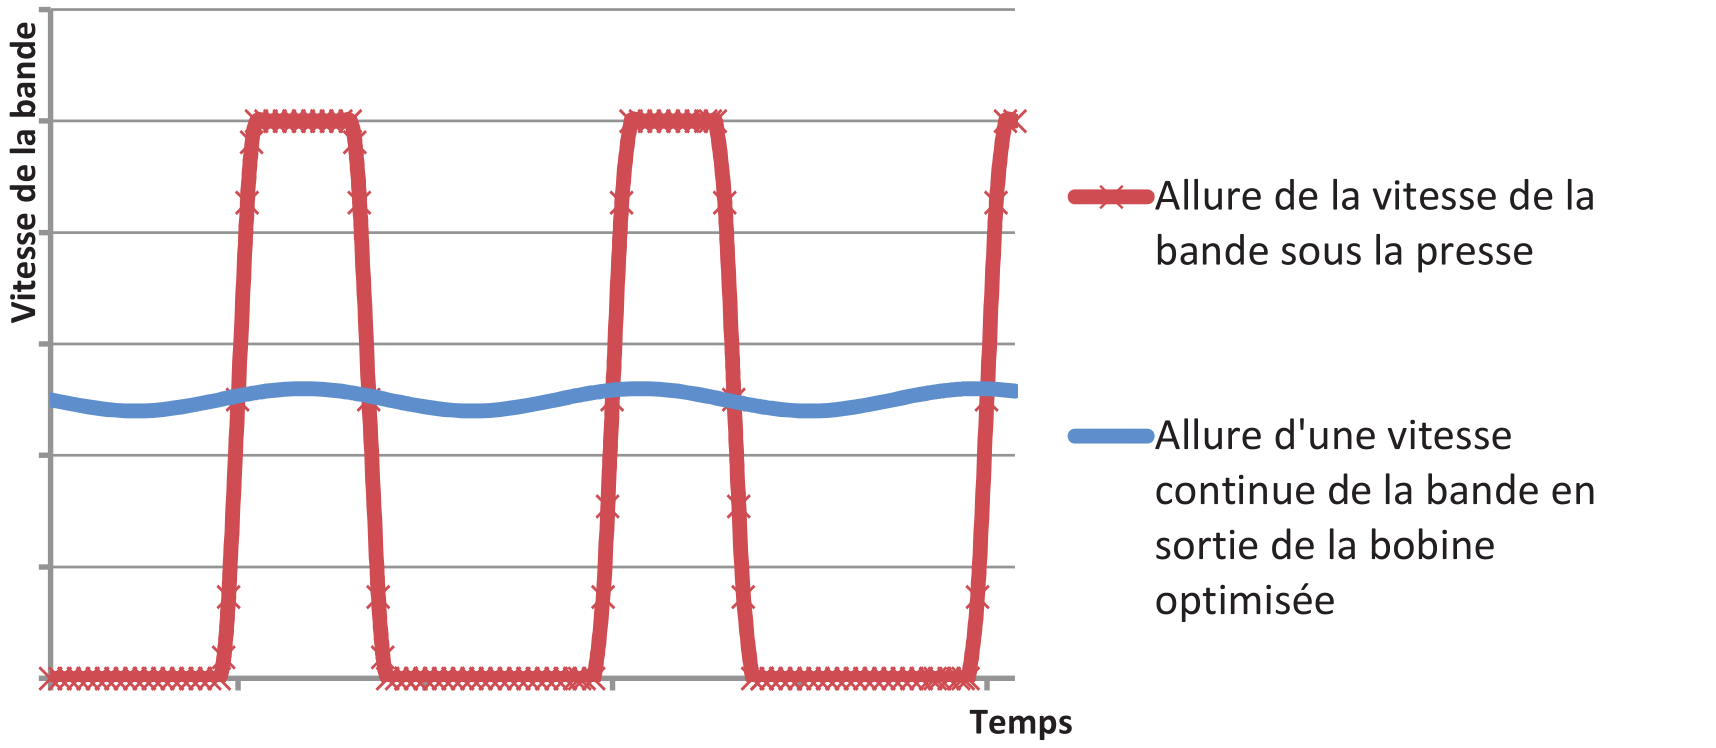
\includegraphics[width=0.7\linewidth]{img/fig7b}
 \caption{Vitesse de la bande}
 \label{fig7b}
\end{figure}

Les quatre types d'architectures les plus utilisées pour les lignes de découpage sont
représentés sur les documents annexes page A2/12 Fig. A-1, A-2, A-3 et A-4.

En fonction du type d'architecture, les différents éléments devront en phase de production (hors
arrêt et mise en place d'une nouvelle bobine) être soit motorisés, soit freinés, soit libres (ni
freinés, ni motorisés).

Le concepteur a besoin de savoir si un élément est motorisé ou freiné.

\question{Pour chaque type d'architecture utilisée, compléter le tableau réponse en indiquant
pour chacun des éléments si la vitesse de la bande est dans cet élément continue ou
discontinue et s'il est motorisé et/ou freiné (mettre des croix dans les cases comme
pour l'exemple). Quelle architecture choisir dans le cas de fortes cadences de production ? Justifier.}

\subsection{Architecture du bras porte-galet 3}

\begin{figure}[!h]
 \centering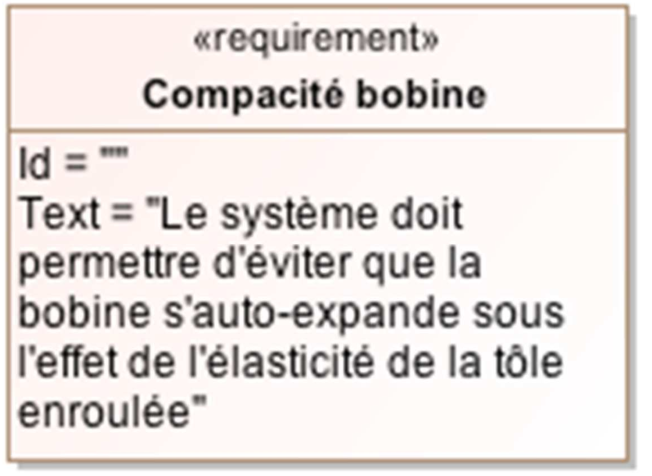
\includegraphics[width=0.3\linewidth]{img/fig8}
 \caption{ Exigence du système \og Compacité bobine \fg}
 \label{fig8}
\end{figure}

Afin de réaliser l'exigence \og Compacité bobine \fg, un bras porte-galet 3 est installé sur le dérouleur (voir annexes page A3/12 Fig.A-5). Sa fonction principale est d'empêcher la bobine de tôle de se dérouler seule à cause du retour élastique, comme une feuille de papier enroulée qui se déroule quand on la relâche. Lors de la mise en place d'une nouvelle bobine de tôle, le bras porte-galet 3 ne doit pas gêner l'opération. Le galet 4 situé à l'extrémité du bras devra toujours être en contact avec la bobine en appliquant un effort minimum de
400N sur celle-ci.

L'effort du galet 4 sur la bobine est obtenu par un vérin pneumatique 1 et 2 et un bras porte-
galet 3. Le vérin pneumatique 1 et 2 est choisi parmi les références habituelles de la société.
Caractéristiques du vérin choisi :
\begin{itemize}
 \item Course notée $C_{verin}$ : 200mm,
 \item $\varnothing$ du piston noté $D_{piston}$ : 80mm,
 \item $\varnothing$ de la tige noté $D_{tige}$ : 25mm,
 \item Pression d'alimentation notée $P_a$ : 0,5MPa,
 \item Rendement du vérin noté $\eta_{verin}$ : 0,9.
\end{itemize}

Dans un premier temps nous allons vérifier si la course du vérin choisi est suffisante.

\paragraph{Étude des différentes positions du bras.} ~\ \\
Sur le document réponse, le système est représenté avec la tige du vérin totalement sortie c'est-à-dire, lorsque le galet 4 est en contact avec une bobine de tôle au diamètre minimum (400 mm).

Les points A, B, C, D, E, F sont les points caractéristiques du système étudié.
\begin{itemize}
 \item Dans la position $P_0$ \og Mise en place d'une bobine \fg (tige de vérin totalement rentrée), on
ajoutera l'indice 0,
 \item Dans la position $P_1$ \og Bobine de diamètre maximum \fg, on ajoutera l'indice 1,
 \item Dans la position $P_2$ \og Bobine de diamètre minimum \fg, on a ajouté l'indice 2.
\end{itemize}

\question{Tracer les points $C_0$ et $D_0$ du bras porte-galet 3 en position $P_0$ \og Mise en place d'une
bobine \fg. Quel est le débattement angulaire total du bras porte-galet 3 ?}

\question{La course du vérin permet-elle de mettre en place une bobine ? Justifier.}

\question{Tracer les points $C_1$ et $D_1$ du bras porte-galet 3 en position $P_1$ \og Bobine de diamètre
maximum \fg. Quel est le débattement angulaire du bras porte-galet 3 pour passer de
la position $P_1$ \og Bobine de diamètre maximum \fg à la position $P_2$ \og Bobine de
diamètre minimum \fg ?}

\question{L'observation de la figure de la question 4 implique une forme particulière à la
silhouette du bras porte-galet 3. Laquelle ? Justifier.}

~\

Dans un second temps nous allons vérifier si l'effort délivré par le vérin choisi est suffisant.

Données sur le bras porte-galet 3 et sur le galet 4 :
\begin{itemize}
 \item Distance (BC) notée $d_{(BC)}$ : 240mm,
 \item Distance (BD) notée $d_{(BD)}$ : 780mm,
 \item Diamètre du galet noté $D_{galet}$ : 75mm.
\end{itemize}

Les repères sont définis sur la Fig. A-8 page A4/12 de l'annexe.

\paragraph{Etude de l'effort presseur du galet 4} ~\ \\
L'étude est réalisée dans la position \og Bobine de diamètre minimum \fg (voir annexes page
A3/12 Fig. A-5)

Les liaisons sont toutes considérées comme parfaites et le poids des pièces est négligé.

L'action mécanique en A du solide 1 sur le solide 0 sera notée : $\overrightarrow{A_{1\rightarrow 0}}$.

Le moment en B de l'action mécanique $\overrightarrow{A_{1\rightarrow 0}}$ sera noté : $\overrightarrow{M_{B,A1\rightarrow 0}}$.

\question{Déterminer la direction de l'effort $\overrightarrow{C_{2\rightarrow 3}}$. Justifier.}

\question{Calculer la norme de l'effort $\overrightarrow{C_{2\rightarrow 3}}$ (expression littérale et résultat numérique).}

\question{Déterminer les directions des efforts $\overrightarrow{F_{5\rightarrow 4}}$ et $\overrightarrow{D_{4\rightarrow 3}}$. Justifier.}

\question{Isoler le bras porte-galet 3 et faire le bilan des actions mécaniques extérieures. Pour
chaque action mécanique, vous indiquerez le point d'application, la direction, le sens
et la norme. Si des données sont inconnues, mettre un point d'interrogation.}

\question{Ecrire l'équation vectorielle d'équilibre des moments du bras porte-galet 3 au point
B.}

\question{Donner l'expression littérale de $\overrightarrow{M_{B,C2\rightarrow 3}}.\overrightarrow{z}$ la projection orthogonale sur l'axe $\overrightarrow{z}$ du moment au point B de $\overrightarrow{C_{2\rightarrow 3}}$ en fonction des caractéristiques du bras porte-galet 3 et de $\overrightarrow{C_{2\rightarrow 3}}.\overrightarrow{y_{C0}}$ la projection orthogonale de $\overrightarrow{C_{2\rightarrow 3}}$ sur l'axe $\overrightarrow{y_{C0}}$.}


\question{Donner l'expression littérale de $\overrightarrow{M_{B,D4\rightarrow 3}}.\overrightarrow{z}$ la projection orthogonale sur l'axe $\overrightarrow{z}$ du moment au point B de $\overrightarrow{D_{4\rightarrow 3}}$ en fonction des caractéristiques du bras porte-galet 3 et de $\overrightarrow{D_{4\rightarrow 3}}.\overrightarrow{y_{D0}}$ la projection orthogonale de $\overrightarrow{D_{4\rightarrow 3}}$ sur l'axe $\overrightarrow{y_{D0}}$.}

\question{Quelle relation existe-t-il entre $\overrightarrow{M_{B,C2\rightarrow 3}}.\overrightarrow{z}$ et $\overrightarrow{M_{B,D4\rightarrow 3}}.\overrightarrow{z}$ ? Compléter la relation du
donnée en utilisant uniquement les signes ($+$ $-$ $\times$ $\div$ $=$ $\neq$ $<$ $>$). }

~\

Les figures Fig. A-11 à A- 13 en annexe pages A6/12 et A7/12 décrivent l'évolution des efforts sur le
bras porte-galet 3 pendant son déplacement. La position de la figure de la question 14 est celle qui est la plus contraignante pour le dimensionnement du galet 4.

Afin de tenir compte d'éventuelles fluctuations de pression dans la chambre du vérin, quel que soit les
résultats précédents, on prendra $\|\overrightarrow{C_{2\rightarrow 3}}\|=2000N$.

\question{Tracer l'effort $\overrightarrow{C_{2\rightarrow 3}}$ (échelle : 10mm $\rightarrow$ 400N).\\
Tracer $\overrightarrow{C_{2\rightarrow 3}}.\overrightarrow{y_{c0}}$ la projection orthogonale de $\overrightarrow{C_{2\rightarrow 3}}$ sur l'axe $\overrightarrow{y_{c0}}$. Donner la
valeur $\overrightarrow{C_{2\rightarrow 3}}.\overrightarrow{y_{c0}}$.\\
A l'aide des relations précédentes (Q9 à Q13) calculer la valeur des expressions suivantes (inscrire uniquement les résultats) :
\begin{itemize}
 \item $\overrightarrow{M_{B,C2\rightarrow 3}}.\overrightarrow{z}$,
 \item $\overrightarrow{M_{B,D4\rightarrow 3}}.\overrightarrow{z}$,
 \item $\overrightarrow{D_{4\rightarrow 3}}.\overrightarrow{y_{D0}}$.
\end{itemize}
Tracer $\overrightarrow{D_{4\rightarrow 3}}.\overrightarrow{y_{D0}}$ la projection orthogonale de $\overrightarrow{D_{4\rightarrow 3}}$ sur l'axe $\overrightarrow{y_{D0}}$.\\
En déduire le tracé de $\overrightarrow{D_{4\rightarrow 3}}$ et donner sa norme $\|\overrightarrow{D_{4\rightarrow 3}}\|$.\\
En vous aidant de la courbe donnée en annexe page A6/12 Fig. A-11, peut-on dire que l'on respecte le cahier des charges (cocher la case correspondante). Justifier.}


\subsection{Etude du mandrin}

Se référer aux annexes, page A10/12 Fig.A-18. En phase utilisation, le mandrin peut se modéliser de la façon suivante:
\begin{figure}[!h]
 \centering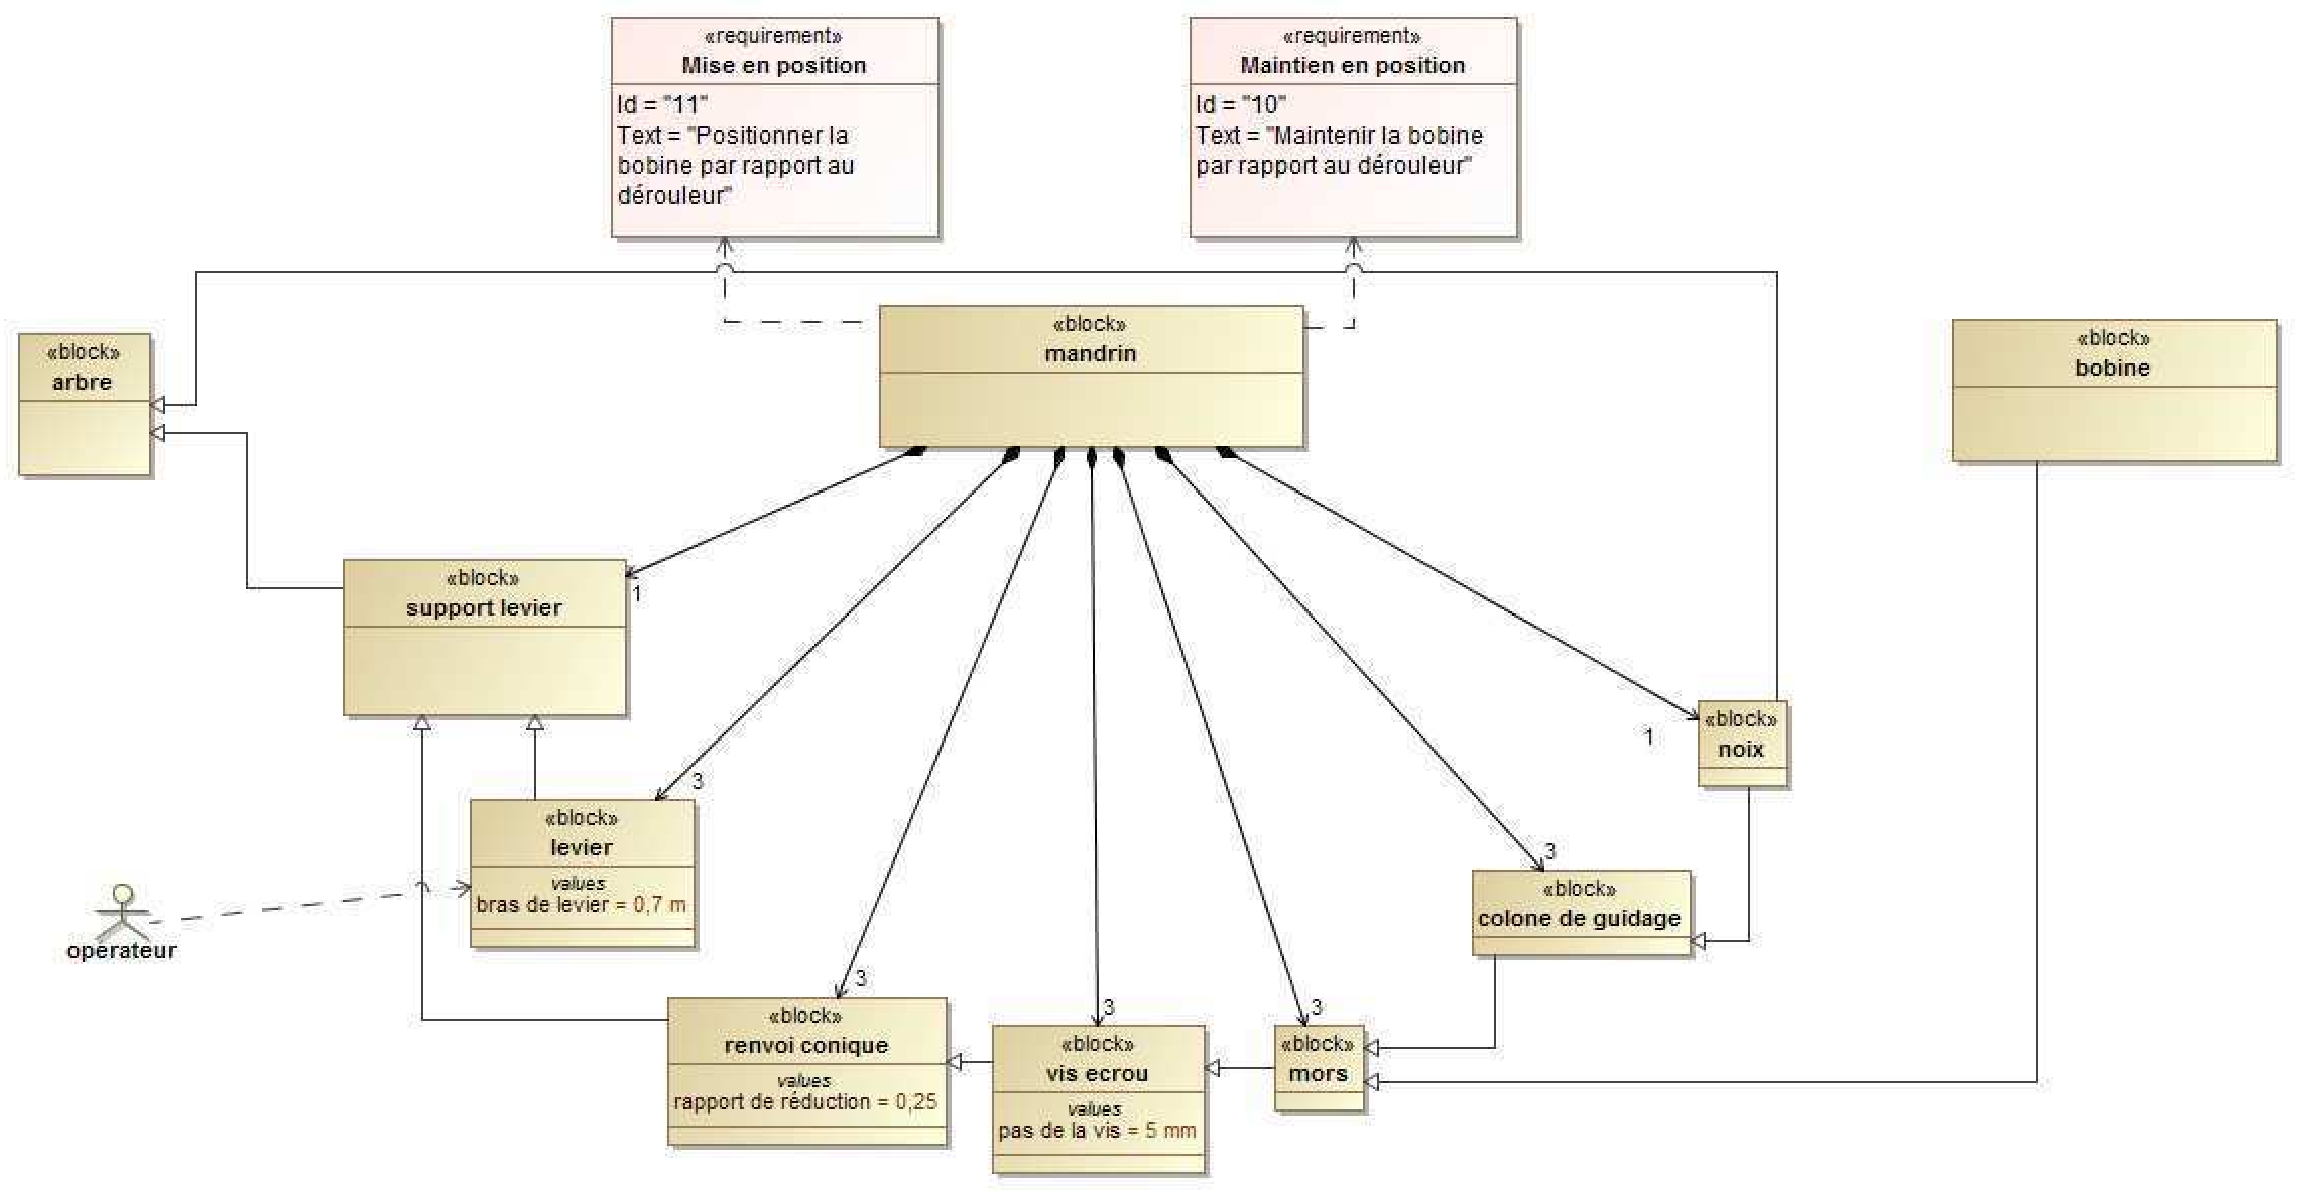
\includegraphics[width=0.9\linewidth]{img/fig12}
 \caption{Diagramme de block du mandrin}
 \label{fig12}
\end{figure}

\paragraph{Constat : } ~\ \\
Lors de l'utilisation du prototype de dérouleur, les opérateurs ont rencontré des difficultés à
man\oe uvrer le mandrin qui met et maintient la bobine en position par rapport à l'arbre (voir
procédure en annexe fig A-19 page A 10/12). Pendant la phase de serrage ou de desserrage
du mandrin, le frein 8 est activé afin d'immobiliser l'arbre 9. Or les efforts des opérateurs sur les
leviers 10 ont parfois mis en rotation l'arbre 9, même avec le frein 8 activé.

\paragraph{Objectif :} ~\ \\
Il s'agit dans un premier temps d'analyser le fonctionnement du mandrin, de faire une étude
statique permettant d'évaluer les efforts et moments mis en jeu pendant les phases de serrage
du mandrin, et de conclure sur l'effort théorique à fournir par l'opérateur.

\subsection{Analyse du fonctionnement du mandrin}

\question{Compléter le schéma cinématique minimal en représentant lisiblement (trais épais,
couleurs,...) les différents symboles des liaisons cinématiques sur les éléments
technologiques qui les constituent.}

\subsection{Etude statique du mandrin en phase \og mise en position \fg}

Il s'agit d'estimer le couple de man\oe uvre,$C_{ma}$, généré par l'effort de l'opérateur sur le levier afin
de mettre les trois mors en contact avec le diamètre intérieur de la bobine.

Données :
\begin{itemize}
 \item Masse maxi de la bobine notée $mb_{max}=500kg$,
 \item Accélération de la pesanteur $g\approx 10 m.s^{-2}$,
 \item Pas de la vis 15 : $p_{vis}=5mm$,
 \item Diamètre de la vis 15 : $\varnothing_{15}=26mm$,
 \item Rapport de réduction du renvoi conique {12,13} : $r_{12,13}=0,25$.
\end{itemize}

~\

Hypothèses :
\begin{itemize}
 \item Les frottements sont négligés, sauf dans le système vis écrou,
 \item Les liaisons sont parfaites,
 \item Toutes les masses sont négligées, sauf celle de la bobine,
 \item Les pièces mobiles du mandrin se déplaçant à vitesse très faible, les effets dynamiques
sont négligés (étude quasi-statique),
 \item La position du mandrin la plus défavorable est représentée sur le document réponse à la question 16. Dans cette position, la bobine repose uniquement sur les deux mors 5 supérieurs. Le troisième mors 5, en position verticale inférieure, n'est pas encore en contact avec la bobine. La position est symétrique.
\end{itemize}

\question{Afin de déterminer les efforts dans chaque mors 5 en fonction du poids de la bobine,
quel(s) solide(s) doit-on isoler ? Tracer les actions mécaniques agissant sur le
système isolé, et donner la relation liant l'intensité des forces de la bobine sur
chaque mors, $\|\overrightarrow{F_{bob\rightarrow mors5-1}}\|$ et $\|\overrightarrow{F_{bob\rightarrow mors5-2}}\|$, en fonction du poids de la bobine $\|\overrightarrow{P_{bob}}\|$.}

L'ensemble $\lbrace$mors5-1 ; écrou14-1$\rbrace$ a été isolé (voir annexes page A10/12 Fig.A-18). Le bilan des efforts extérieurs ne fait apparaitre que trois torseurs :

$\left\{\tau_{bob\rightarrow mors5-1}\right\}=\left\{\begin{array}{cc}
0 & 0\\
-F_{mors5-1\rightarrow bob} & 0\\
0 & 0
\end{array}\right\}_{K,R_5(0,x_5,y_5,z_5)}$

$\left\{\tau_{col\rightarrow mors5-1}\right\}=\left\{\begin{array}{cc}
X_{CM} & L_{CM}\\
0 & M_{CM}\\
Z_{CM} & N_{CM}
\end{array}\right\}_{J,R_5(0,x_5,y_5,z_5)}$\\

$\left\{\tau_{vis\rightarrow ecrou}\right\}=\left\{\begin{array}{cc}
X_{VE} & L_{VE}\\
Y_{VE} & M_{VE}\\
Z_{VE} & N_{VE}
\end{array}\right\}_{I,R_5(0,x_5,y_5,z_5)}$, avec $M_{VE}=k_1.Y_{VE}$ ($k_1$ sera déterminé plus loin).

On donne (en mm):$\overrightarrow{IJ}=95.\overrightarrow{x_5}$, $\overrightarrow{IK}=220.\overrightarrow{x_5}-45.\overrightarrow{y_5}$.

\question{Quelle composante de ces torseurs représente la valeur de l'effort axial dans la vis $\|\overrightarrow{F_{a-vis}}\|$?}

\question{Compléter le document réponse après avoir analysé les torseurs donnés ci-dessus. \\
Identifier quelle(s) projection(s) de quel(s) théorème(s) permet d'exprimer rapidement l'effort axial dans la vis, $\|\overrightarrow{F_{a-vis}}\|$, en fonction de l'effort du mors5-1 sur la bobine, $F_{mors5-1\rightarrow bob}$.}

\question{Déduire des questions précédentes la relation liant l'effort axial dans la vis $\|\overrightarrow{F_{a-vis}}\|$ au poids de la bobine $P_{bob}$.}

~\

Le document annexe page A12/12 Fig. 21 précise les différentes caractéristiques des
systèmes vis-écrous utilisés.

\question{Exprimer le couple d'entrainement axial dans la vis, $C_{a-vis}$ (N.m), en fonction de $F_{a-vis}$ (N), du pas de la vis $p_{vis}$ (mm) et de son rendement $\eta_{vis}$. \\
Calculer la valeur de la constante $k_1$ telle que $C_{a-vis}=k_1.F_{a-vis}$ et préciser son unité.}

\question{Quelle relation lie le moment axial $C_{a-vis}$ dans une vis et le couple unitaire sur la roue
conique, $C_{roue-unit}$. Justifier votre réponse.}

\question{Déduire des questions précédentes la valeur du couple man\oe uvre, $C_{ma}$, généré par
l'effort de l'opérateur sur le levier pour soulever la bobine.}

\question{Après un relevé de dimension(s) sur le plan donné en annexe page A9/12 Fig. 17,
évaluer l'effort que doit exercer l'opérateur $F_{op}$ sur un seul levier pour soulever la
bobine. Que pensez-vous de cette valeur ?}

\newpage

\section{Dessin d'étude de construction mécanique}

Il est demandé aux candidats des dessins qui doivent traduire sans ambiguïté leurs intentions
de conception. Pour cela, ils sont invités à faire preuve de rigueur dans leur tracé (en particulier,
l'utilisation d'une règle ne pourra être que conseillée) et à donner toutes les précisions qu'ils
jugeront pertinentes afin de permettre aux correcteurs d'évaluer la pertinence de leurs
solutions. La lisibilité des solutions est prise en compte dans l'évaluation.

\subsection{Présentation du support de travail}

\begin{figure}[!h]
 \centering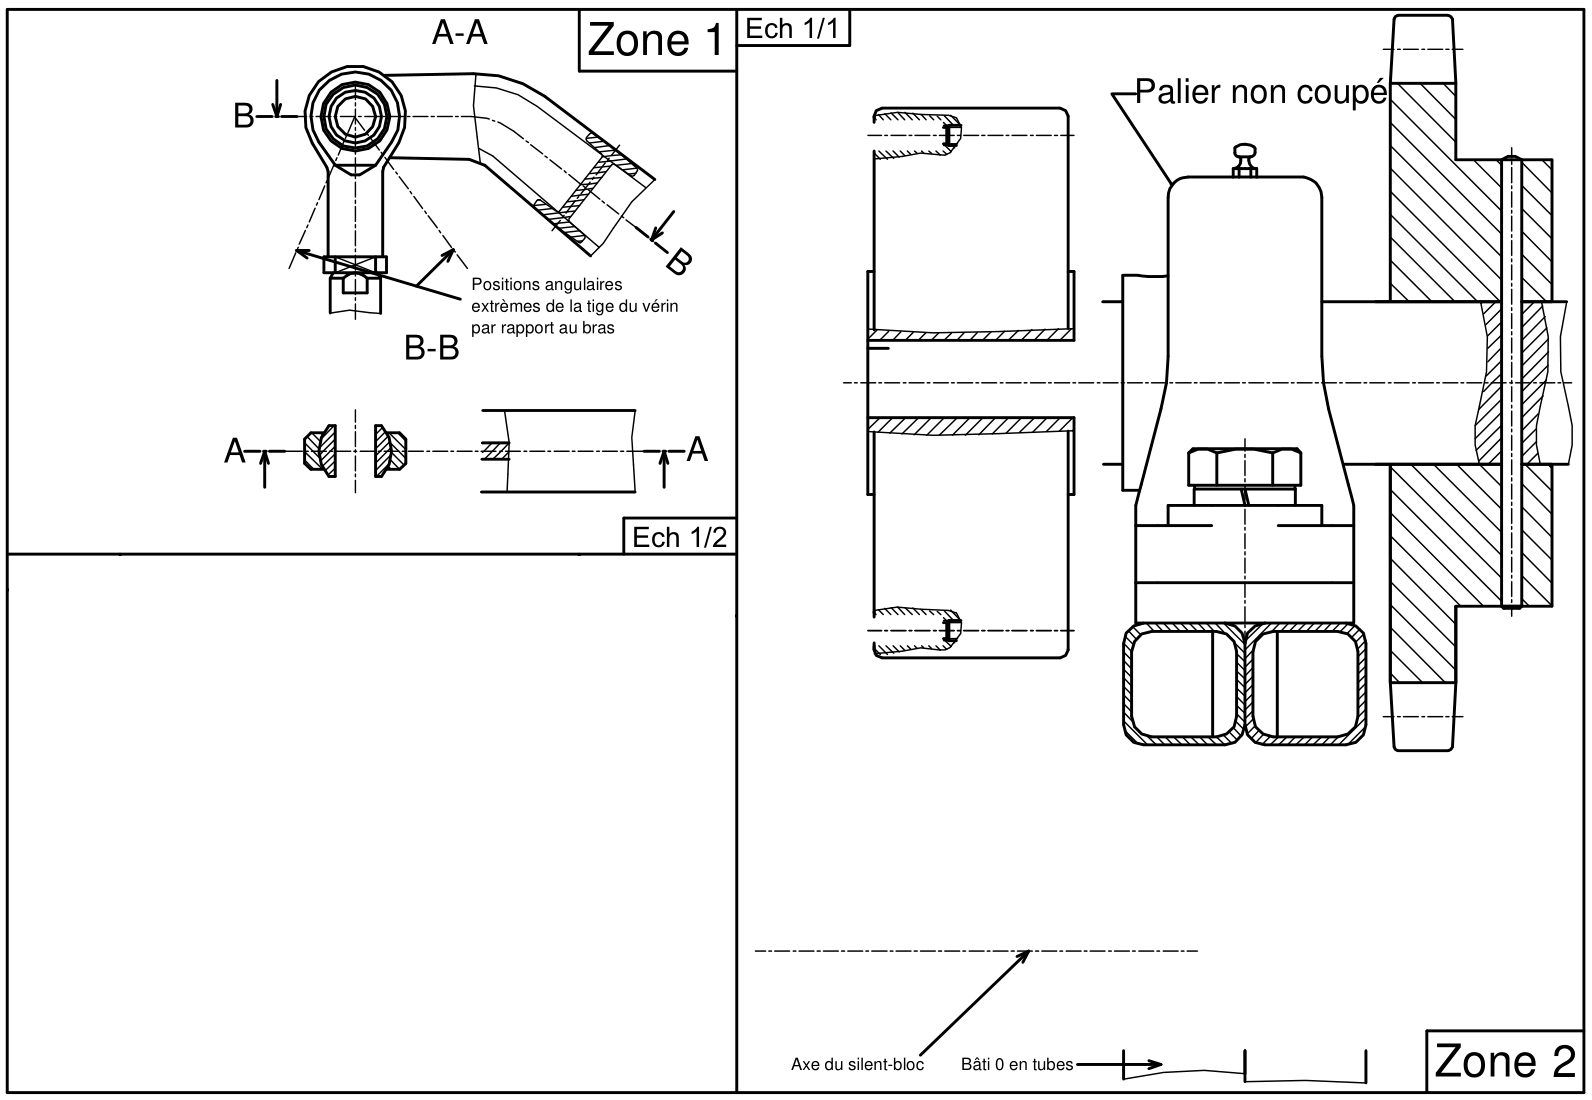
\includegraphics[width=0.7\linewidth]{img/fig13}
 \caption{Calque}
 \label{fig13}
\end{figure}

\vspace{-30pt}

\subsection{Conception du bras porte-galet 3}

\paragraph{Présentation du travail}

Dans cette partie, nous allons terminer la conception du bras porte-galet 3.

Cette partie concerne deux zones du calque:
\begin{itemize}
 \item Zone 1 : Liaison rotule démontable entre la tige de vérin 2 et le bras porte-galet 3,
 \item Zone 2 : Liaison pivot démontable entre le bâti 0 et le bras porte-galet 3.
\end{itemize}

La section retenue pour le bras porte-galet 3 est la section 2 Fig. 12 ci-après. Seule la cote h
évolue toute au long du bras afin d'avoir une poutre iso contrainte.

Le bras porte-galet 3 sera réalisé en une seule pièce, moulée en sable en acier GS335. La
forme du bras porte-galet 3 retenue est représentée ci-après. Le profil en I du bras porte-galet
reste invariable tout au long de celui-ci mis à part la hauteur h.

\newpage

Au niveau des zones à définir, des bossages, nervures ou toutes autres formes compatibles
avec le processus de moulage et avec le plan de joint défini ci-après, sont réalisables.

\begin{figure}[!h]
 \centering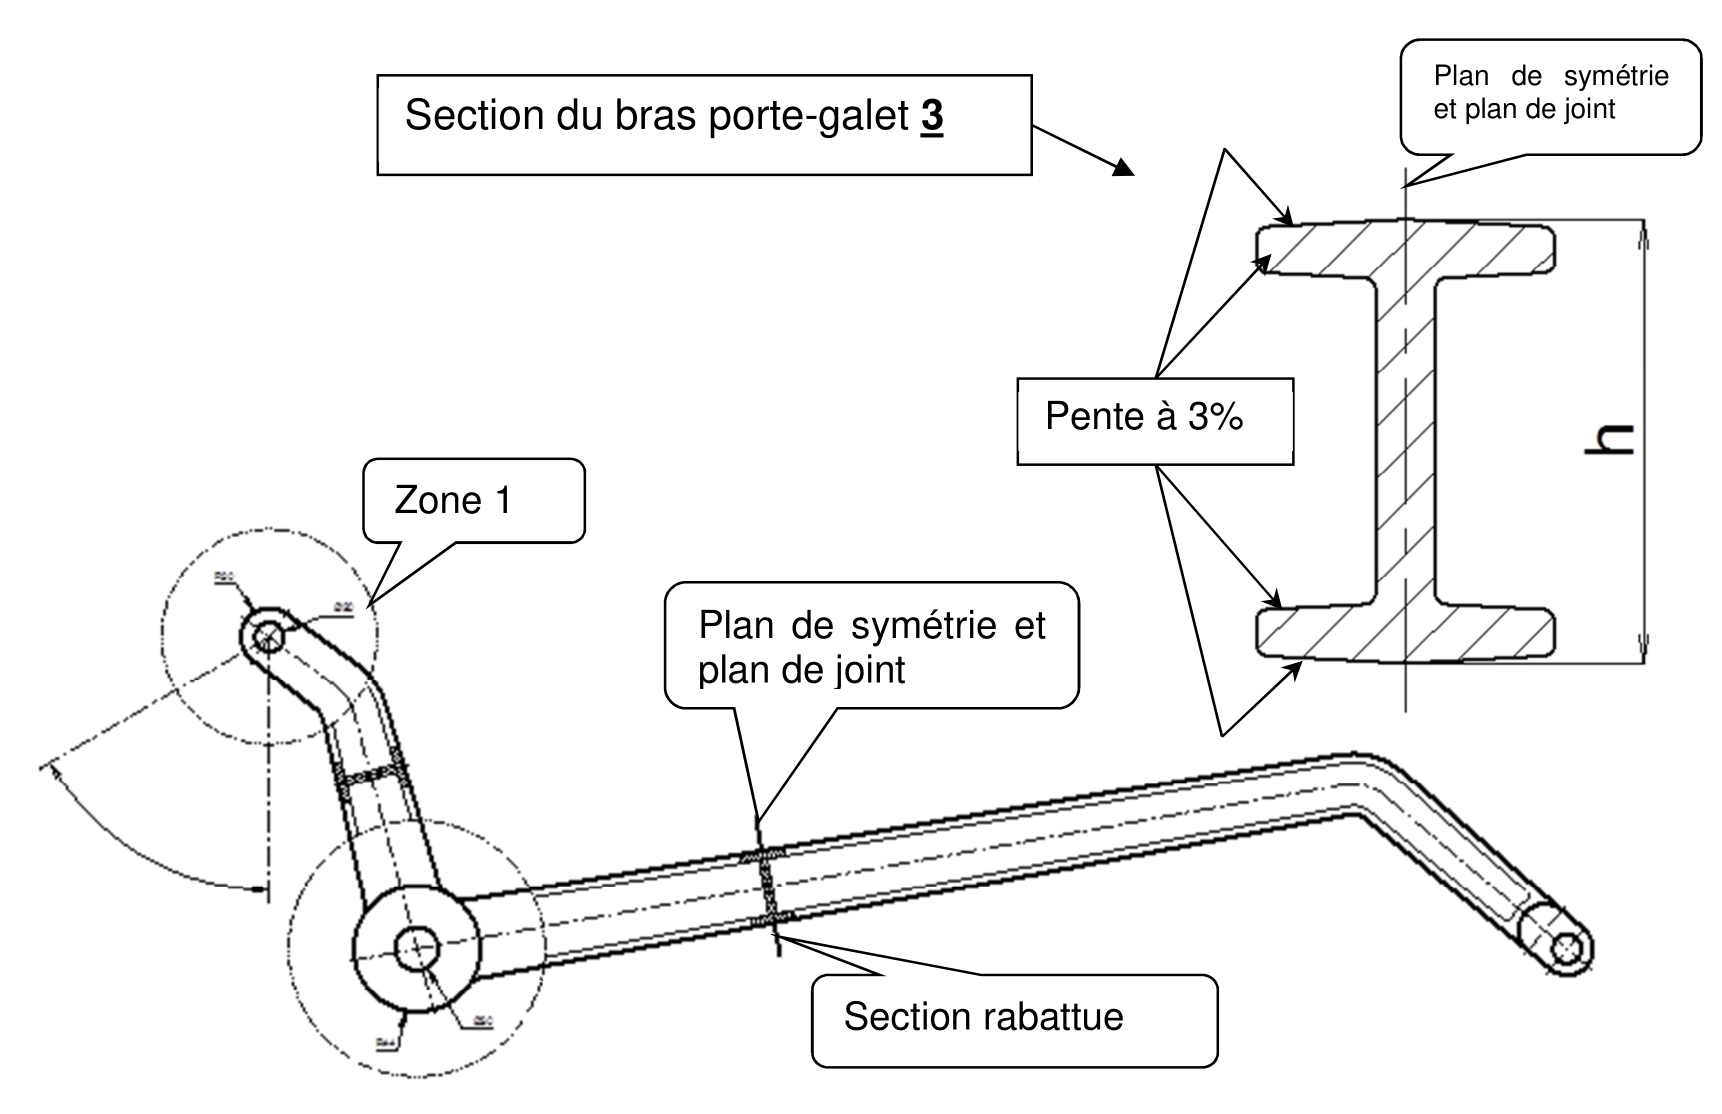
\includegraphics[width=0.7\linewidth]{img/fig14}
 \caption{Forme générale du bras porte-galet 3}
 \label{fig14}
\end{figure}

\paragraph{Travail à réaliser : Liaison rotule Tige de vérin 2-Bras porte-galet 3} ~\ \\
\question{Représenter une solution technique permettant la liaison pivot glissant démontable entre la tige de vérin 2 et le bras porte-galet 3. L'embout de la tige de vérin est un élément standard (voir annexe page A7/12 fig A 14). Définir les formes locales du bras porte-galet 3 et les pièces permettant de réaliser la liaison entre celui-ci etl'embout à rotule. Mettre en place les ajustements normalisés nécessaires à la liaison.}


\subsection{Conception de la mise en place du frein à poudre.}

\paragraph{Présentation du travail}

Dans cette partie, nous allons concevoir l'installation du frein à poudre sur le dérouleur.

Cette modification engendre différents changements sur le prototype précédemment réalisé
(voir annexes page A10/12 Fig A 18).

Cette conception est à réaliser dans la zone 2 du calque.

Sur le prototype, la liaison pivot entre l'arbre principal 9 et le bâti 0 mécano-soudé, était réalisée
par deux paliers auto aligneurs. Cette solution est conservée.

Dans la nouvelle conception, le frein permanent est retiré. Le bâti 0 ne sera pas modifié.

Le nouveau système sera composé pour l'essentiel d'un frein à poudre. Le frein à poudre
utilisé, est de référence Mérobel FAT 350. La faible vitesse de rotation ainsi le facteur de
charge faible du frein pendant le fonctionnement, permet son installation sans système de
refroidissement. (Voir annexes page A8/12 Fig 16).

\paragraph{Travail à réaliser}

Dans la zone 2 du calque, le frein à poudre et le palier auto aligneur coté frein sont déjà
représentés.

Le frein à poudre est installé à l'extrémité de l'arbre 9.

L'arrêt en rotation du frein à poudre par rapport au bâti 0 sera réalisé par l'intermédiaire d'un
élément élastique \og Silent bloc \fg comme le préconise le constructeur.

Le \og Silent bloc \fg choisi a pour référence SR 5040 chez AURA INSDUSTRIE. Il sera installé à
140 mm de l'axe de l'arbre 9 sur l'axe pré dessiné.

Les éléments de visserie d'assemblage peuvent être soit représentés selon les normes soit
spécifiés uniquement par un trait d'axe avec une indication (exemple : 3Vis CHC M10 à 120°).

\question{Réaliser une liaison glissière entre le frein à poudre (moyeu) et l'arbre principal.}

\question{Réaliser l'arrêt en rotation du frein à poudre par rapport au bâti 0. Pour cela il sera
nécessaire de :
\begin{itemize}
 \item Définir le flasque permettant de relier le frein à poudre au \og Silent bloc SR 5040 \fg,
 \item Implanter le \og Silent bloc SR 5040 \fg,
 \item Définir l'équerre de fixation du \og Silent bloc SR 5040 \fg au bâti 0. Cette équerre sera fixée sur le bâti 0 avec les boulons du palier auto aligneur coté frein,
 \item Fixer le \og Silent bloc SR 5040 \fg au flasque et à l'équerre,
 \item Mettre en place les ajustements normalisés nécessaires.
\end{itemize}}

\begin{table}
\begin{tabular}{|c|l|c|c|}
\hline
$C_{verin}$ & Course du vérin du bras porte galet & 3 & 200mm \\ \hline
$D_{piston}$ & Diamètre du piston du vérin du bras porte galet 3 &80& mm \\ \hline
$D_{tige}$ & Diamètre de la tige du vérin du bras porte galet 3 &25& mm \\ \hline
$P_a$ & Pression d'alimentation du vérin du bras porte galet 3 &0,5& MPa \\ \hline
$\eta_{verin}$ & Rendement du vérin du bras porte galet 3 &0,9& \\ \hline
$D_{galet}$ & Diamètre extérieur du galet 4 &75& mm \\ \hline
$\overrightarrow{C_{2\rightarrow 3}}$ & Effort de la tige du vérin 2 sur le bras porte galet 3 en C & &  \\ \hline
$\overrightarrow{F_{5\rightarrow 4}}$ & Effort de la bobine de tôle 5 sur le galet 4 en F & &  \\ \hline
$\overrightarrow{D_{4\rightarrow 3}}$ & Effort du galet 4 sur le bras porte galet 3 en D & &  \\ \hline
$B_{R-palier}$ & Charge radiale sur un des deux paliers auto aligneur de la liaison 3/0 & & \\ \hline
$C_{ma}$ & Couple de man\oe uvre généré par l'opérateur & &  \\ \hline
$g$ & Accélération de la pesanteur & 10 & $m.s^{-2}$  \\ \hline
$\overrightarrow{F_{bob/mors 1}}$ & Effort de la bobine 5 sur le mors i (1?i?3) & &  \\ \hline
$P_{bob}$ & Poids de la bobine & &  \\ \hline
$\overrightarrow{F_{a-vis}}$ & Effort axial dans la vis de man\oe uvre des mors & &  \\ \hline
$C_{a-vis}$ & Couple axial dans la vis de man\oe uvre des mors & &  \\ \hline
$p_{vis}$ & Pas de la vis de man\oe uvre des mors &5& mm  \\ \hline
$\eta_{vis}$ & Rendement de la vis de man\oe uvre des mors & &  \\ \hline
$F_{op}$ & Effort de l'opérateur & &  \\ \hline
$mb_{max}$ & Masse maximale de la bobine 5 &500& kg \\ \hline
$Db_{int\ min}$ & Diamètre intérieur minimum de la bobine de tôle 5 & 400 & mm \\ \hline
$Db_{ext\ max}$ & Diamètre extérieur maximum de la bobine de tôle 5 & 1000 & mm  \\ \hline
$Lb_{max}$ & Largeur maximum de la bobine de tôle 5 & 200 & mm  \\ \hline
$V_{tole\ max}$ & Vitesse linéaire maximum de déroulement de la tôle & 0,2 & $m.s^{-1}$ \\ \hline
$D_{stop\ max}$ & Distance d'arrêt maximum de la tôle & 0,25 & m \\ \hline
$C_{f\ max}$ & Couple de freinage maximum & &  \\ \hline
\end{tabular}
\caption{Tableau récapitulatif des données et des notations principales du sujet}
\end{table}

\newpage

\pagestyle{empty}


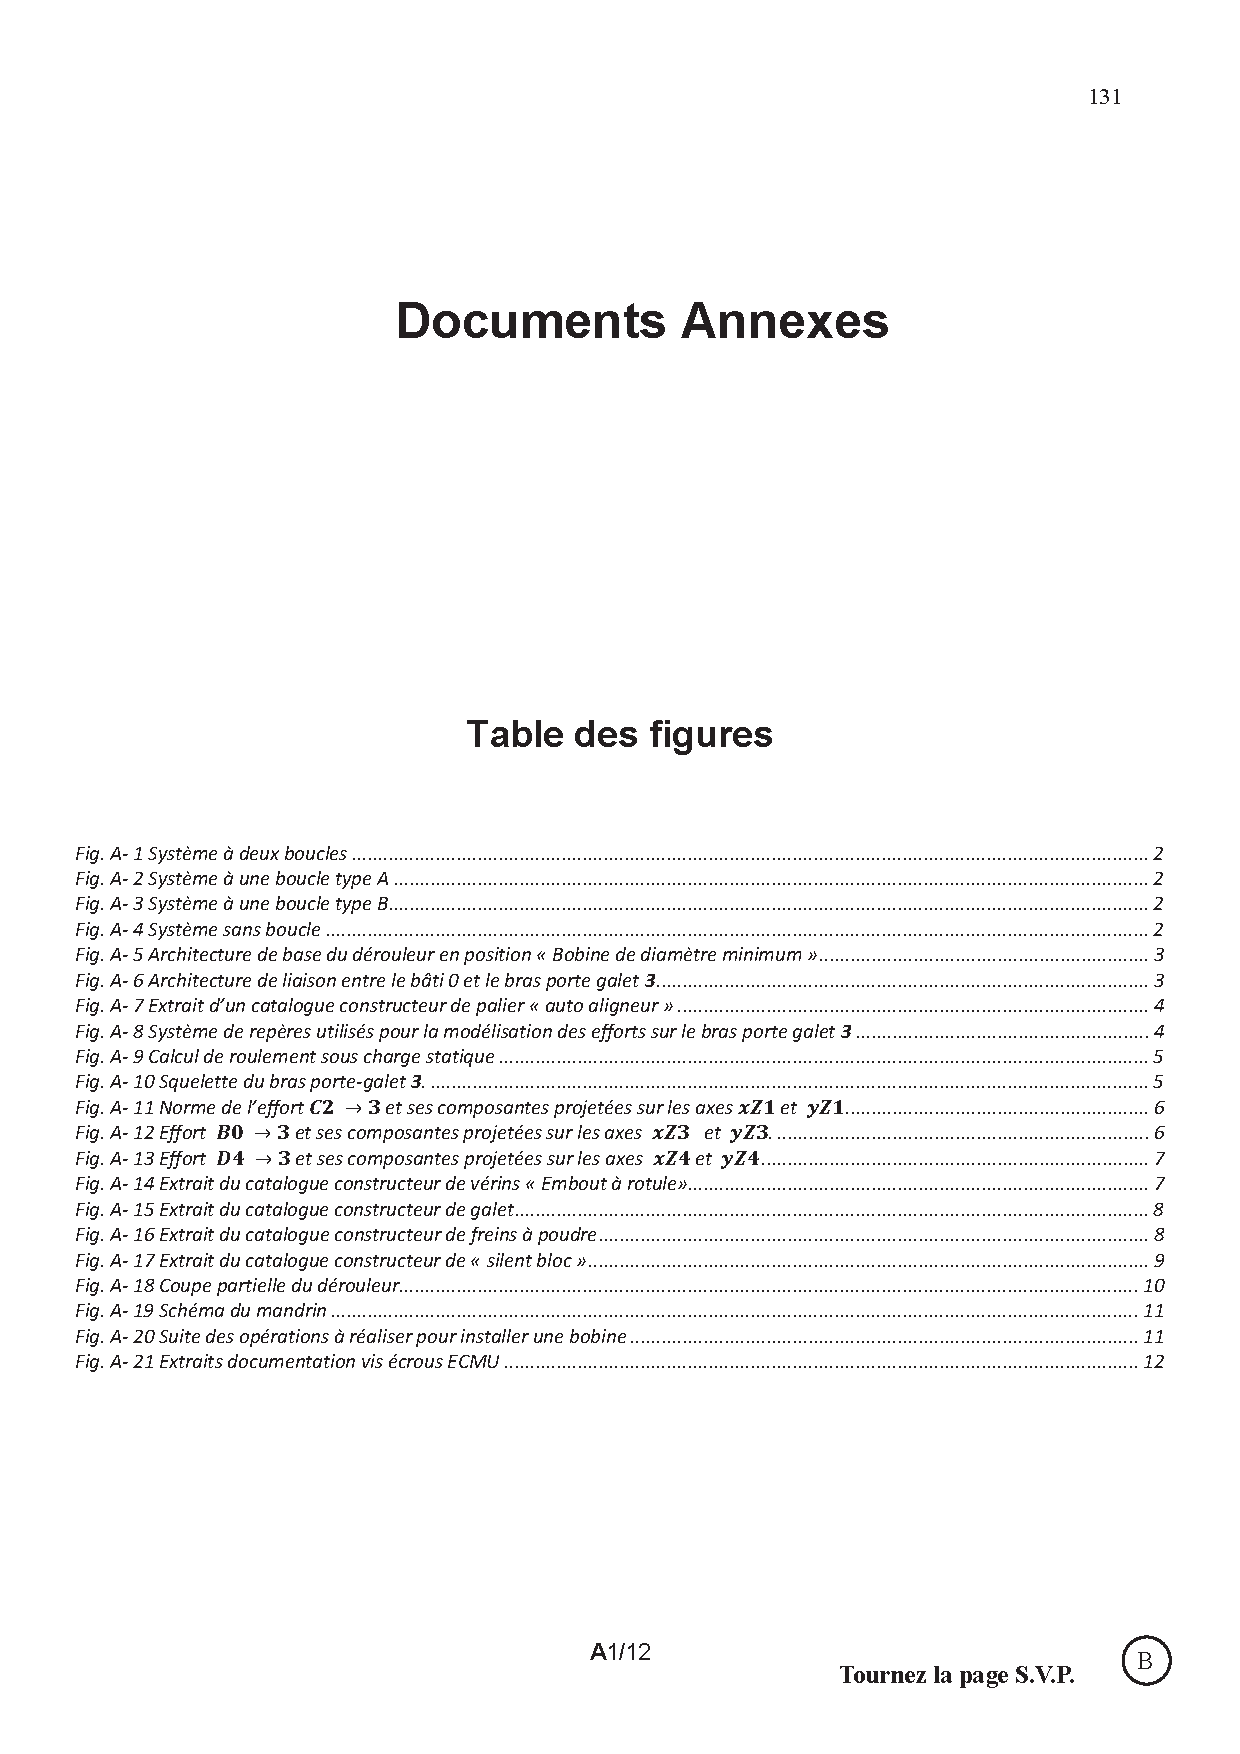
\includepdf[pages={-},templatesize={210mm}{297mm},offset=0cm -1cm]{img/annexes.pdf}
\newpage
\cleardoublepage

\pagestyle{documentreponse}

\section{Documents réponse}

\reponse{1}{\ifdef{\public}{
\begin{tabular}{|c|c|c|c|c|c|}
\hline
Rep. & Système d'alimentation & Question & Dérouleur & Redresseur & Amenage \\ \hline
\multirow{4}{*}{1} & \multirow{4}{*}{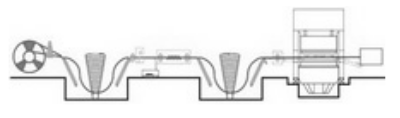
\includegraphics[width=0.3\linewidth]{img/dr1_1}} & Vit. discontinue & & & X \\ \cline{3-6}
 & & Vit. continue & X & X & \\ \cline{3-6}
 & & Motorisé & & & \\ \cline{3-6}
 & & Freiné & & & \\ \hline
\multirow{4}{*}{2} & \multirow{4}{*}{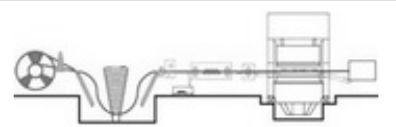
\includegraphics[width=0.3\linewidth]{img/dr1_2}} & Vit. discontinue & & & \\ \cline{3-6}
 & & Vit. continue & & & \\ \cline{3-6}
 & & Motorisé & & & \\ \cline{3-6}
 & & Freiné & & & \\ \hline
\multirow{4}{*}{3} & \multirow{4}{*}{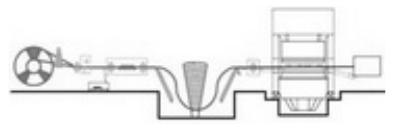
\includegraphics[width=0.3\linewidth]{img/dr1_3}} & Vit. discontinue & & & \\ \cline{3-6}
 & & Vit. continue & & & \\ \cline{3-6}
 & & Motorisé & & & \\ \cline{3-6}
 & & Freiné & & & \\ \hline
\multirow{4}{*}{4} & \multirow{4}{*}{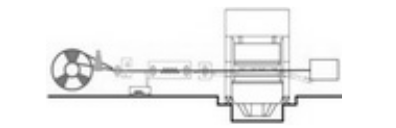
\includegraphics[width=0.3\linewidth]{img/dr1_4}} & Vit. discontinue & & & \\ \cline{3-6}
 & & Vit. continue & & & \\ \cline{3-6}
 & & Motorisé & & & \\ \cline{3-6}
 & & Freiné & & & \\ \hline
\end{tabular}

Choix du type d'architecture:

Justification: }{
\begin{tabular}{|c|c|c|c|c|c|}
\hline
Rep. & Système d'alimentation & Question & Dérouleur & Redresseur & Amenage \\ \hline
\multirow{4}{*}{1} & \multirow{4}{*}{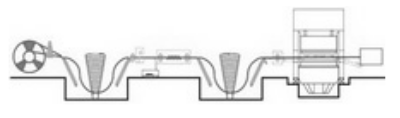
\includegraphics[width=0.3\linewidth]{img/dr1_1}} & Vit. discontinue & & & X \\ \cline{3-6}
 & & Vit. continue & X & X & \\ \cline{3-6}
 & & Motorisé & X & X & X \\ \cline{3-6}
 & & Freiné & & & \\ \hline
\multirow{4}{*}{2} & \multirow{4}{*}{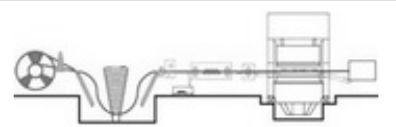
\includegraphics[width=0.3\linewidth]{img/dr1_2}} & Vit. discontinue & & X & X \\ \cline{3-6}
 & & Vit. continue & X & & \\ \cline{3-6}
 & & Motorisé & X & & X \\ \cline{3-6}
 & & Freiné & & & \\ \hline
\multirow{4}{*}{3} & \multirow{4}{*}{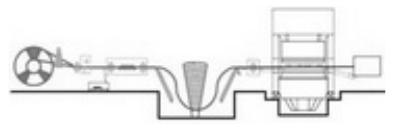
\includegraphics[width=0.3\linewidth]{img/dr1_3}} & Vit. discontinue & & & X \\ \cline{3-6}
 & & Vit. continue & X & X & \\ \cline{3-6}
 & & Motorisé & & X & X \\ \cline{3-6}
 & & Freiné & & & \\ \hline
\multirow{4}{*}{4} & \multirow{4}{*}{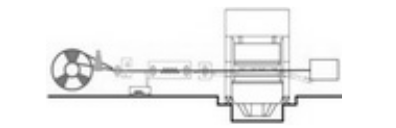
\includegraphics[width=0.3\linewidth]{img/dr1_4}} & Vit. discontinue & X & X & X \\ \cline{3-6}
 & & Vit. continue & & & \\ \cline{3-6}
 & & Motorisé & X & & X \\ \cline{3-6}
 & & Freiné & X & & \\ \hline
\end{tabular}

Choix du type d'architecture: \textbf{1}.

Justification: Cette solution permet de garder une vitesse constante, donc il y a peu d'à-coups grâce aux boucles.
}}

\reponse{1}{\ifdef{\public}{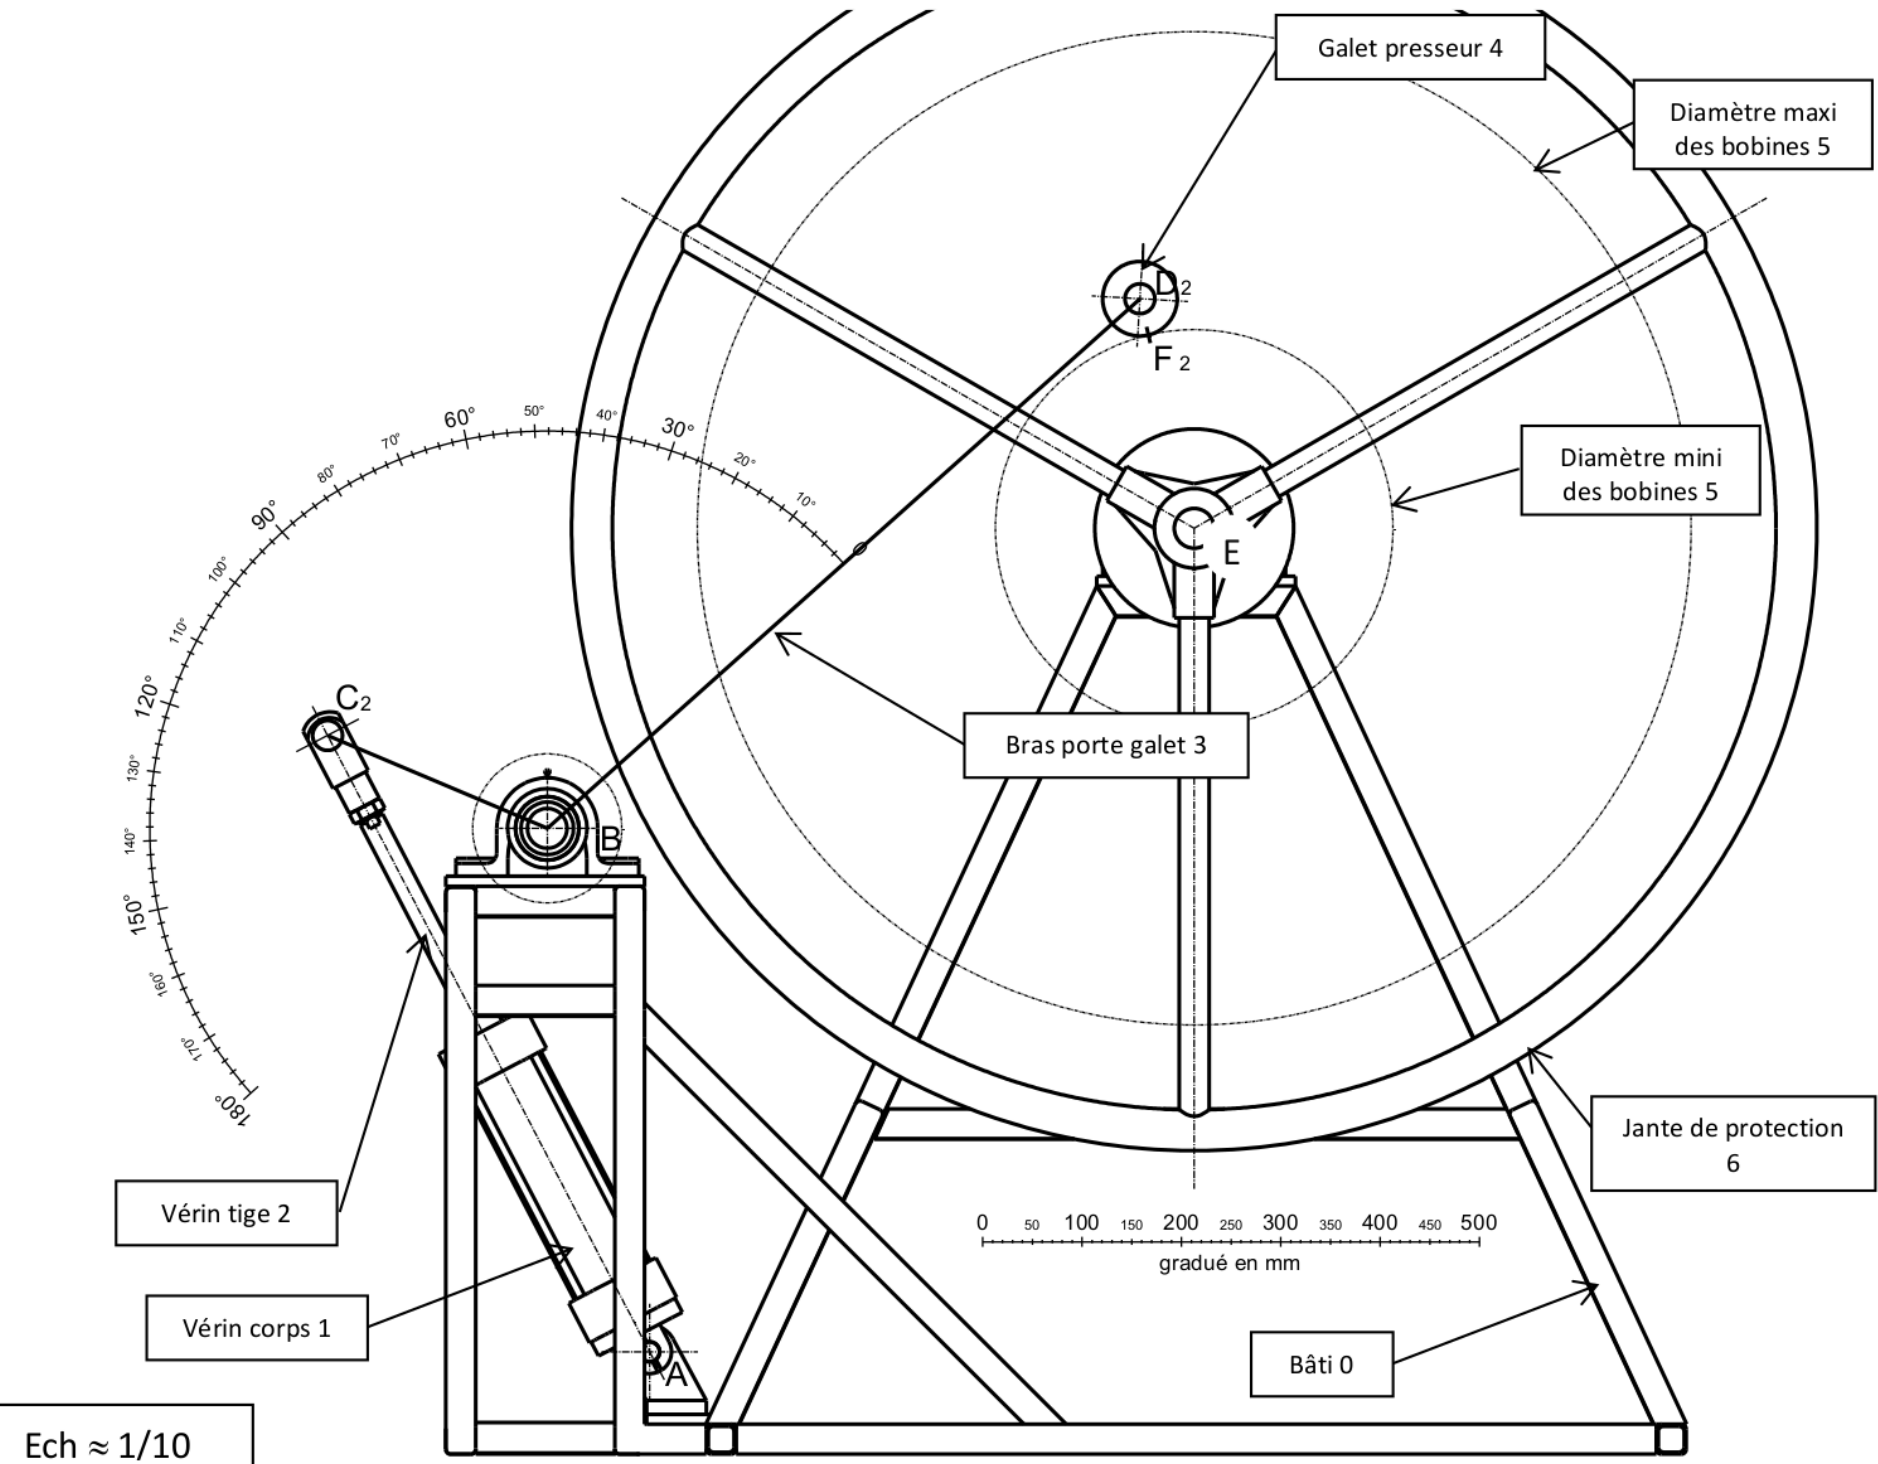
\includegraphics[width=0.8\linewidth]{img/dr2} \\ Le débattement angulaire total du bras porte galet 3 est :}
{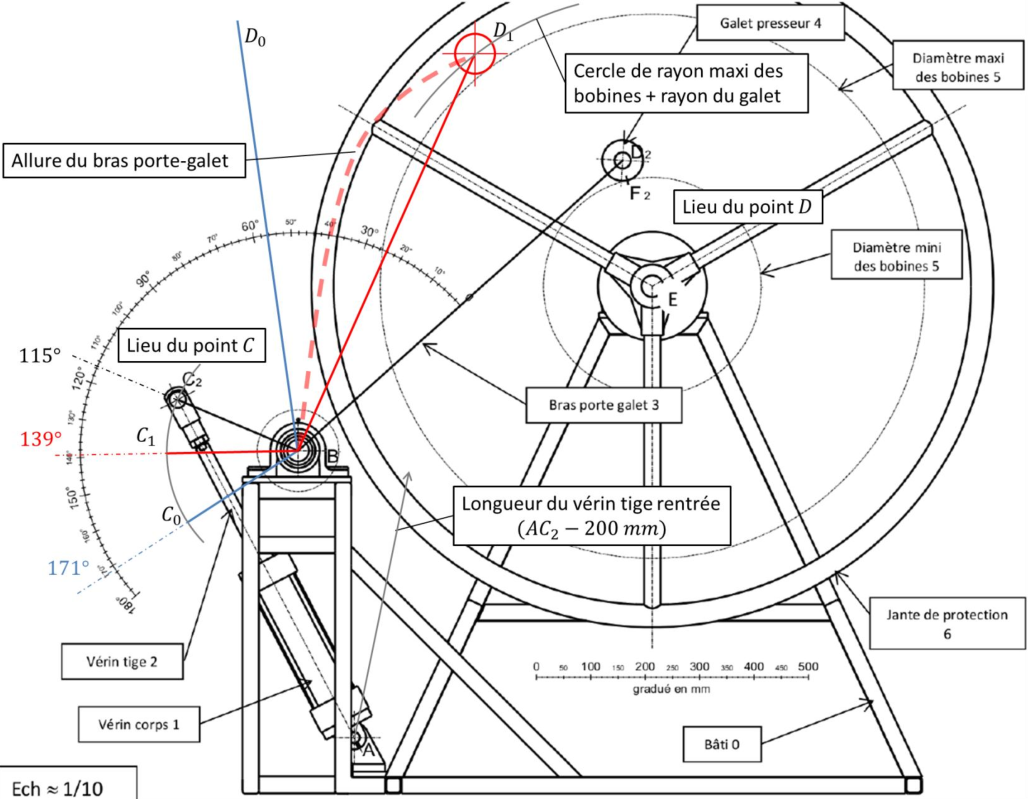
\includegraphics[width=0.78\linewidth]{img/dr2_cor} \\ Le débattement angulaire total du bras porte galet 3 est : 56\degree}}

\newpage

\reponse{1}{\ifdef{\public}{\vspace{0.5cm}}
{Dans la position $P_0$, le bras n'est plus en contact et la bobine n'interfère pas avec la jante, la bobine peut être mise en place.}}

\reponse{1}{\ifdef{\public}{Faire les constructions sur la figure de la question 2. \\ Débattement angulaire du bras porte-galet 3 entre la position P1 et la position P2:}
{Faire les constructions  sur la figure de la question 2. \\ Débattement angulaire du bras porte-galet 3 entre la position P1 et la position P2: 24 \degree}}

\reponse{1}{\ifdef{\public}{\vspace{1cm}}{Il y a une interférence entre la bobine au diamètre max et la droite $BD_1$, il faudra ainsi adapter le bras.}

\reponse{1}{\ifdef{\public}{\vspace{1cm}}{Direction AC. L'ensemble $\lbrace$ 1+2 $\rbrace$ est soumis à 2 glisseurs en A et C.}}

\reponse{1}{\ifdef{\public}{$\|\overrightarrow{C_{2\rightarrow 3}}\|=$\hspace{4cm}, $\|\overrightarrow{C_{2\rightarrow 3}}\|=$}{$\|\overrightarrow{C_{2\rightarrow 3}}\|=P_a.\pi.\frac{D^2_{piston}}{4}.\eta_{piston}$, $\|\overrightarrow{C_{2\rightarrow 3}}\|=2160N.$}}

\reponse{1}{\ifdef{\public}{\vspace{1cm}}{$EF_2$ et $F_2D_2$, contact galet/bobine radial, donc $EF_2$, le galet est soumis à deux actions en $F_2$ et $D_2$, donc $F_2D_2$.}}

\reponse{1}{\ifdef{\public}{
\begin{center}
\begin{tabular}{|c|c|c|c|c|}
\hline
Action mécanique & Point d'application & Direction & Sens & Norme \\ \hline
  &  &   &   & \\ \hline
  &  &   &   & \\ \hline
  &  &   &   & \\ \hline
  &  &   &   & \\ \hline
\end{tabular}
\end{center}
}{
\begin{center}
\begin{tabular}{|c|c|c|c|c|}
\hline
Action mécanique & Point d'application & Direction & Sens & Norme \\ \hline
$\overrightarrow{C_{2\rightarrow 3}}$ & C & $AC_2$ & $A\rightarrow C_2$ & $P_a.\pi.\frac{D^2_{piston}}{4}$ \\ \hline
$\overrightarrow{D_{4\rightarrow 3}}$ & D & $F_2D_2$ & ? & ? \\ \hline
$\overrightarrow{B_{0\rightarrow 3}}$ & B & ? & ? & ? \\ \hline
  &  &   &   & \\ \hline
\end{tabular}
\end{center}}}

\reponse{1}{\ifdef{\public}{\vspace{1cm}}{$\overrightarrow{M_{B,C2\rightarrow 3}}+\overrightarrow{M_{B,D4\rightarrow 3}}+\overrightarrow{M_{B,B0\rightarrow 3}}=\overrightarrow{0}$}}

\reponse{1}{\ifdef{\public}{$\overrightarrow{M_{B,C2\rightarrow 3}}.\overrightarrow{z}=$}{$\overrightarrow{M_{B,C2\rightarrow 3}}.\overrightarrow{z}=-d_{(BC)}.\overrightarrow{C_{2\rightarrow 3}}.\overrightarrow{y_{C0}}$}}

\reponse{1}{\ifdef{\public}{$\overrightarrow{M_{B,D4\rightarrow 3}}.\overrightarrow{z}=$}{$\overrightarrow{M_{B,D4\rightarrow 3}}.\overrightarrow{z}-d_{(BD)}.\overrightarrow{D_{4\rightarrow 3}}.\overrightarrow{y_{D0}}$}}

\reponse{1}{\ifdef{\public}{\vspace{2cm}}{$\overrightarrow{M_{B,C2\rightarrow 3}}.\overrightarrow{z}=-\overrightarrow{M_{B,D4\rightarrow 3}}.\overrightarrow{z}$}}

\reponse{1}{\ifdef{\public}{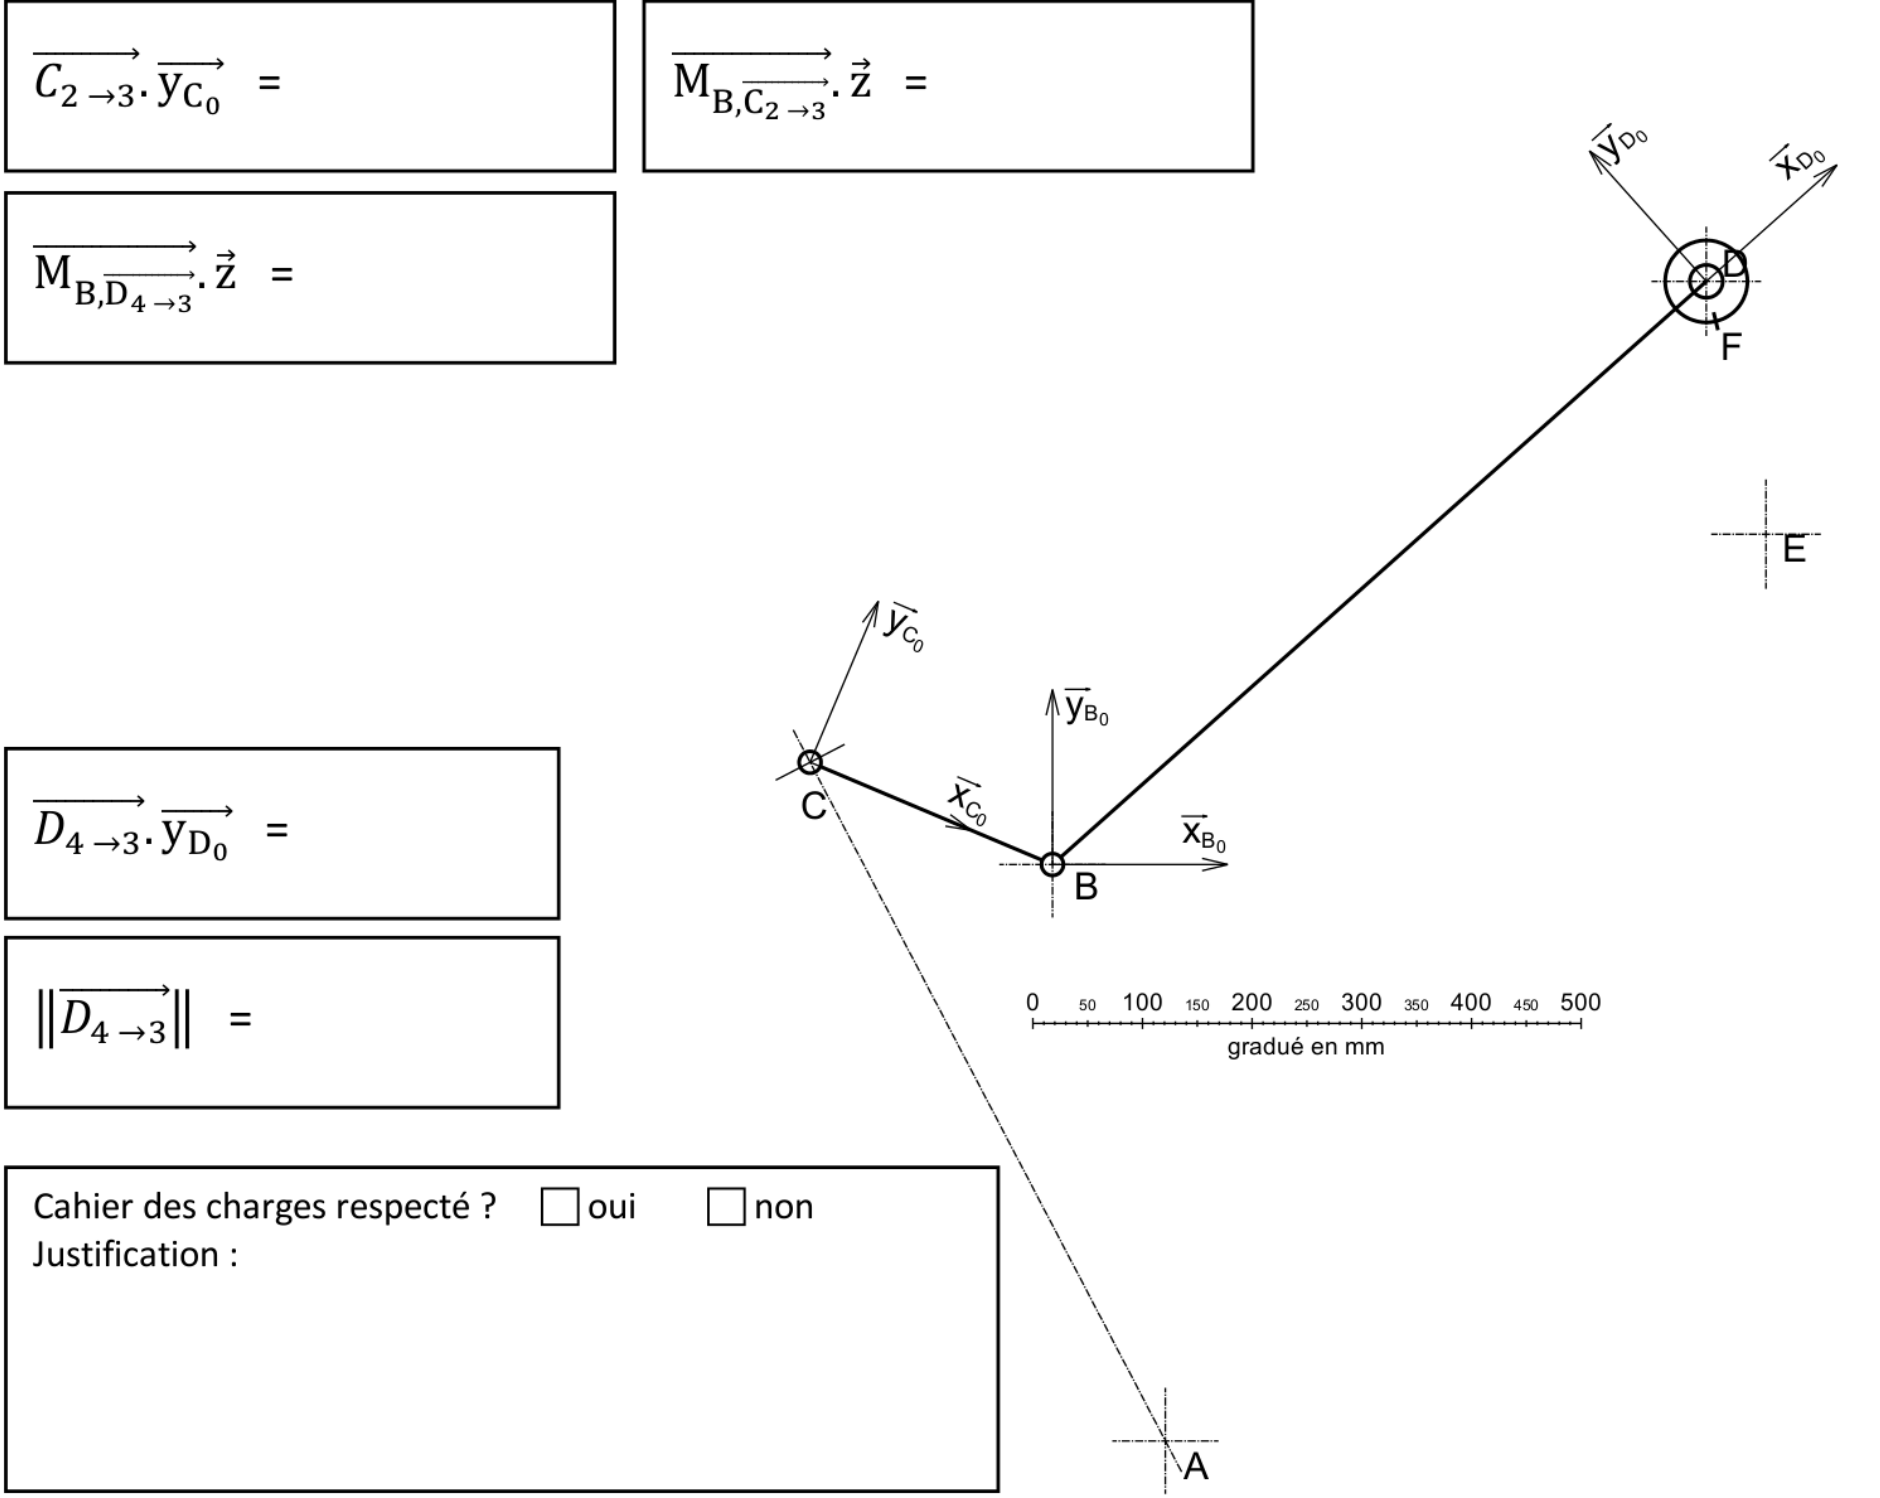
\includegraphics[width=0.9\linewidth]{img/dr14}}{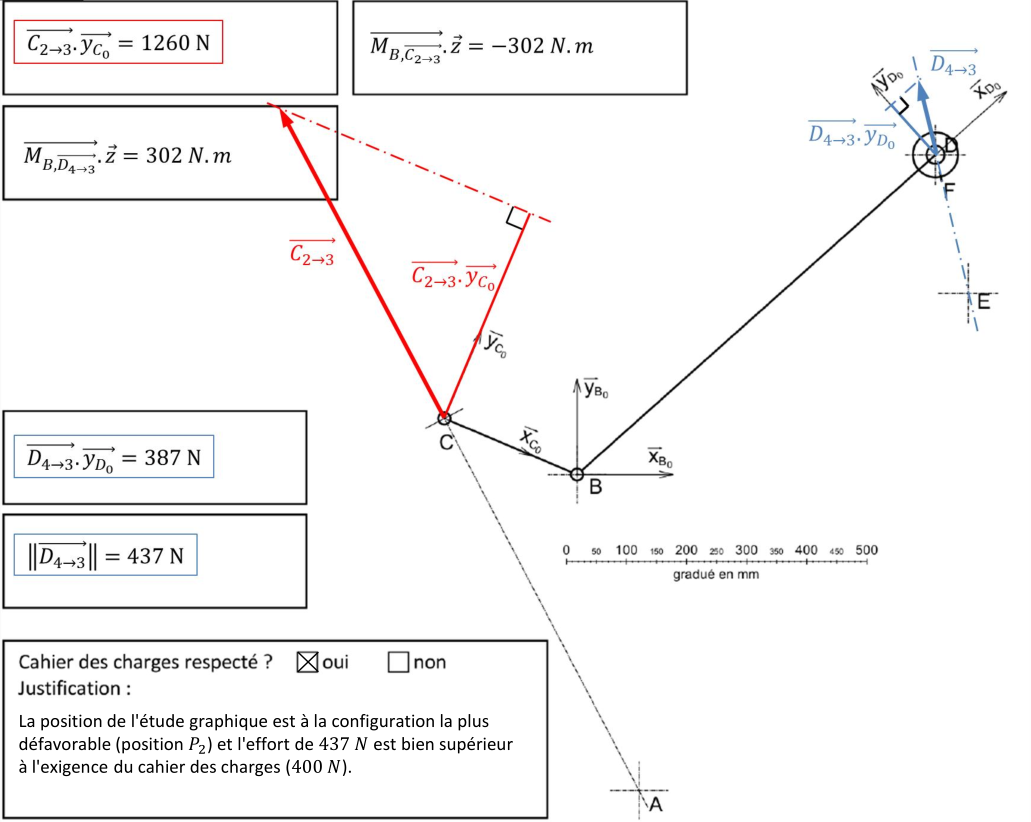
\includegraphics[width=0.9\linewidth]{img/dr14_cor}}}

\reponse{1}{\ifdef{\public}{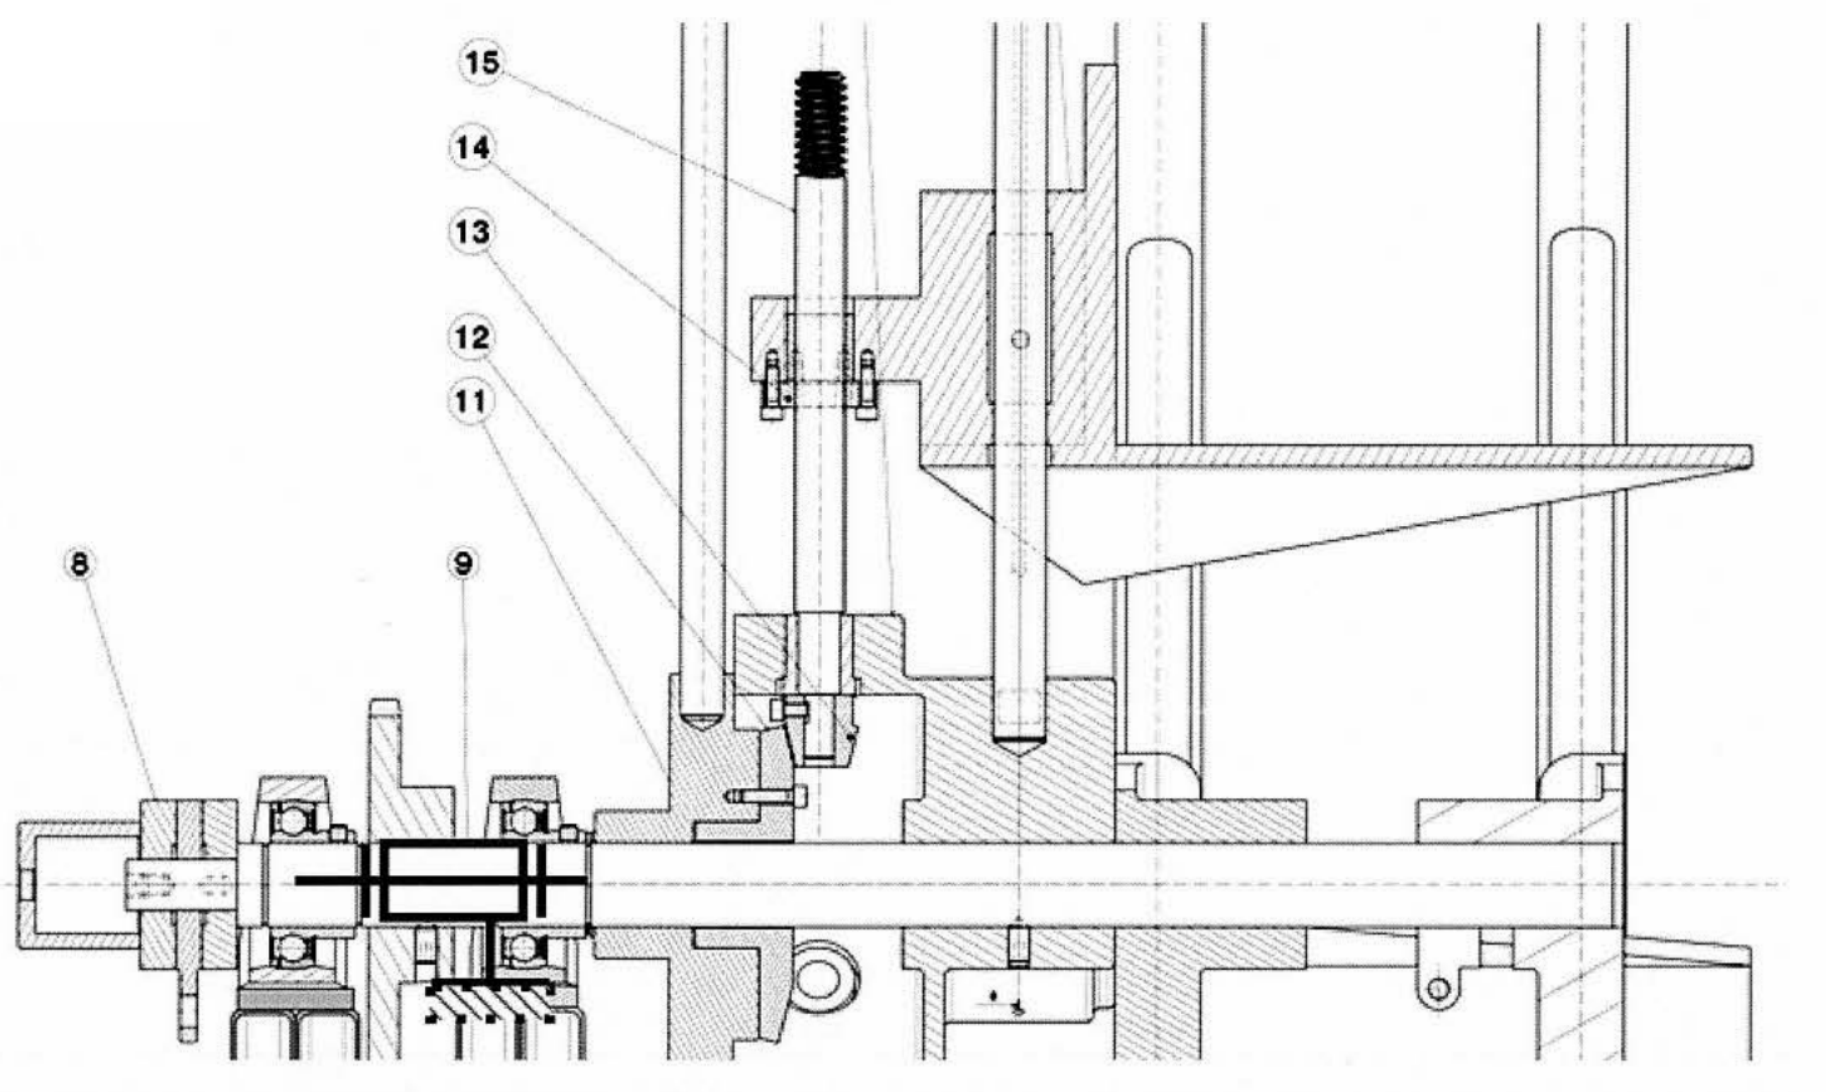
\includegraphics[width=0.9\linewidth]{img/dr20}}{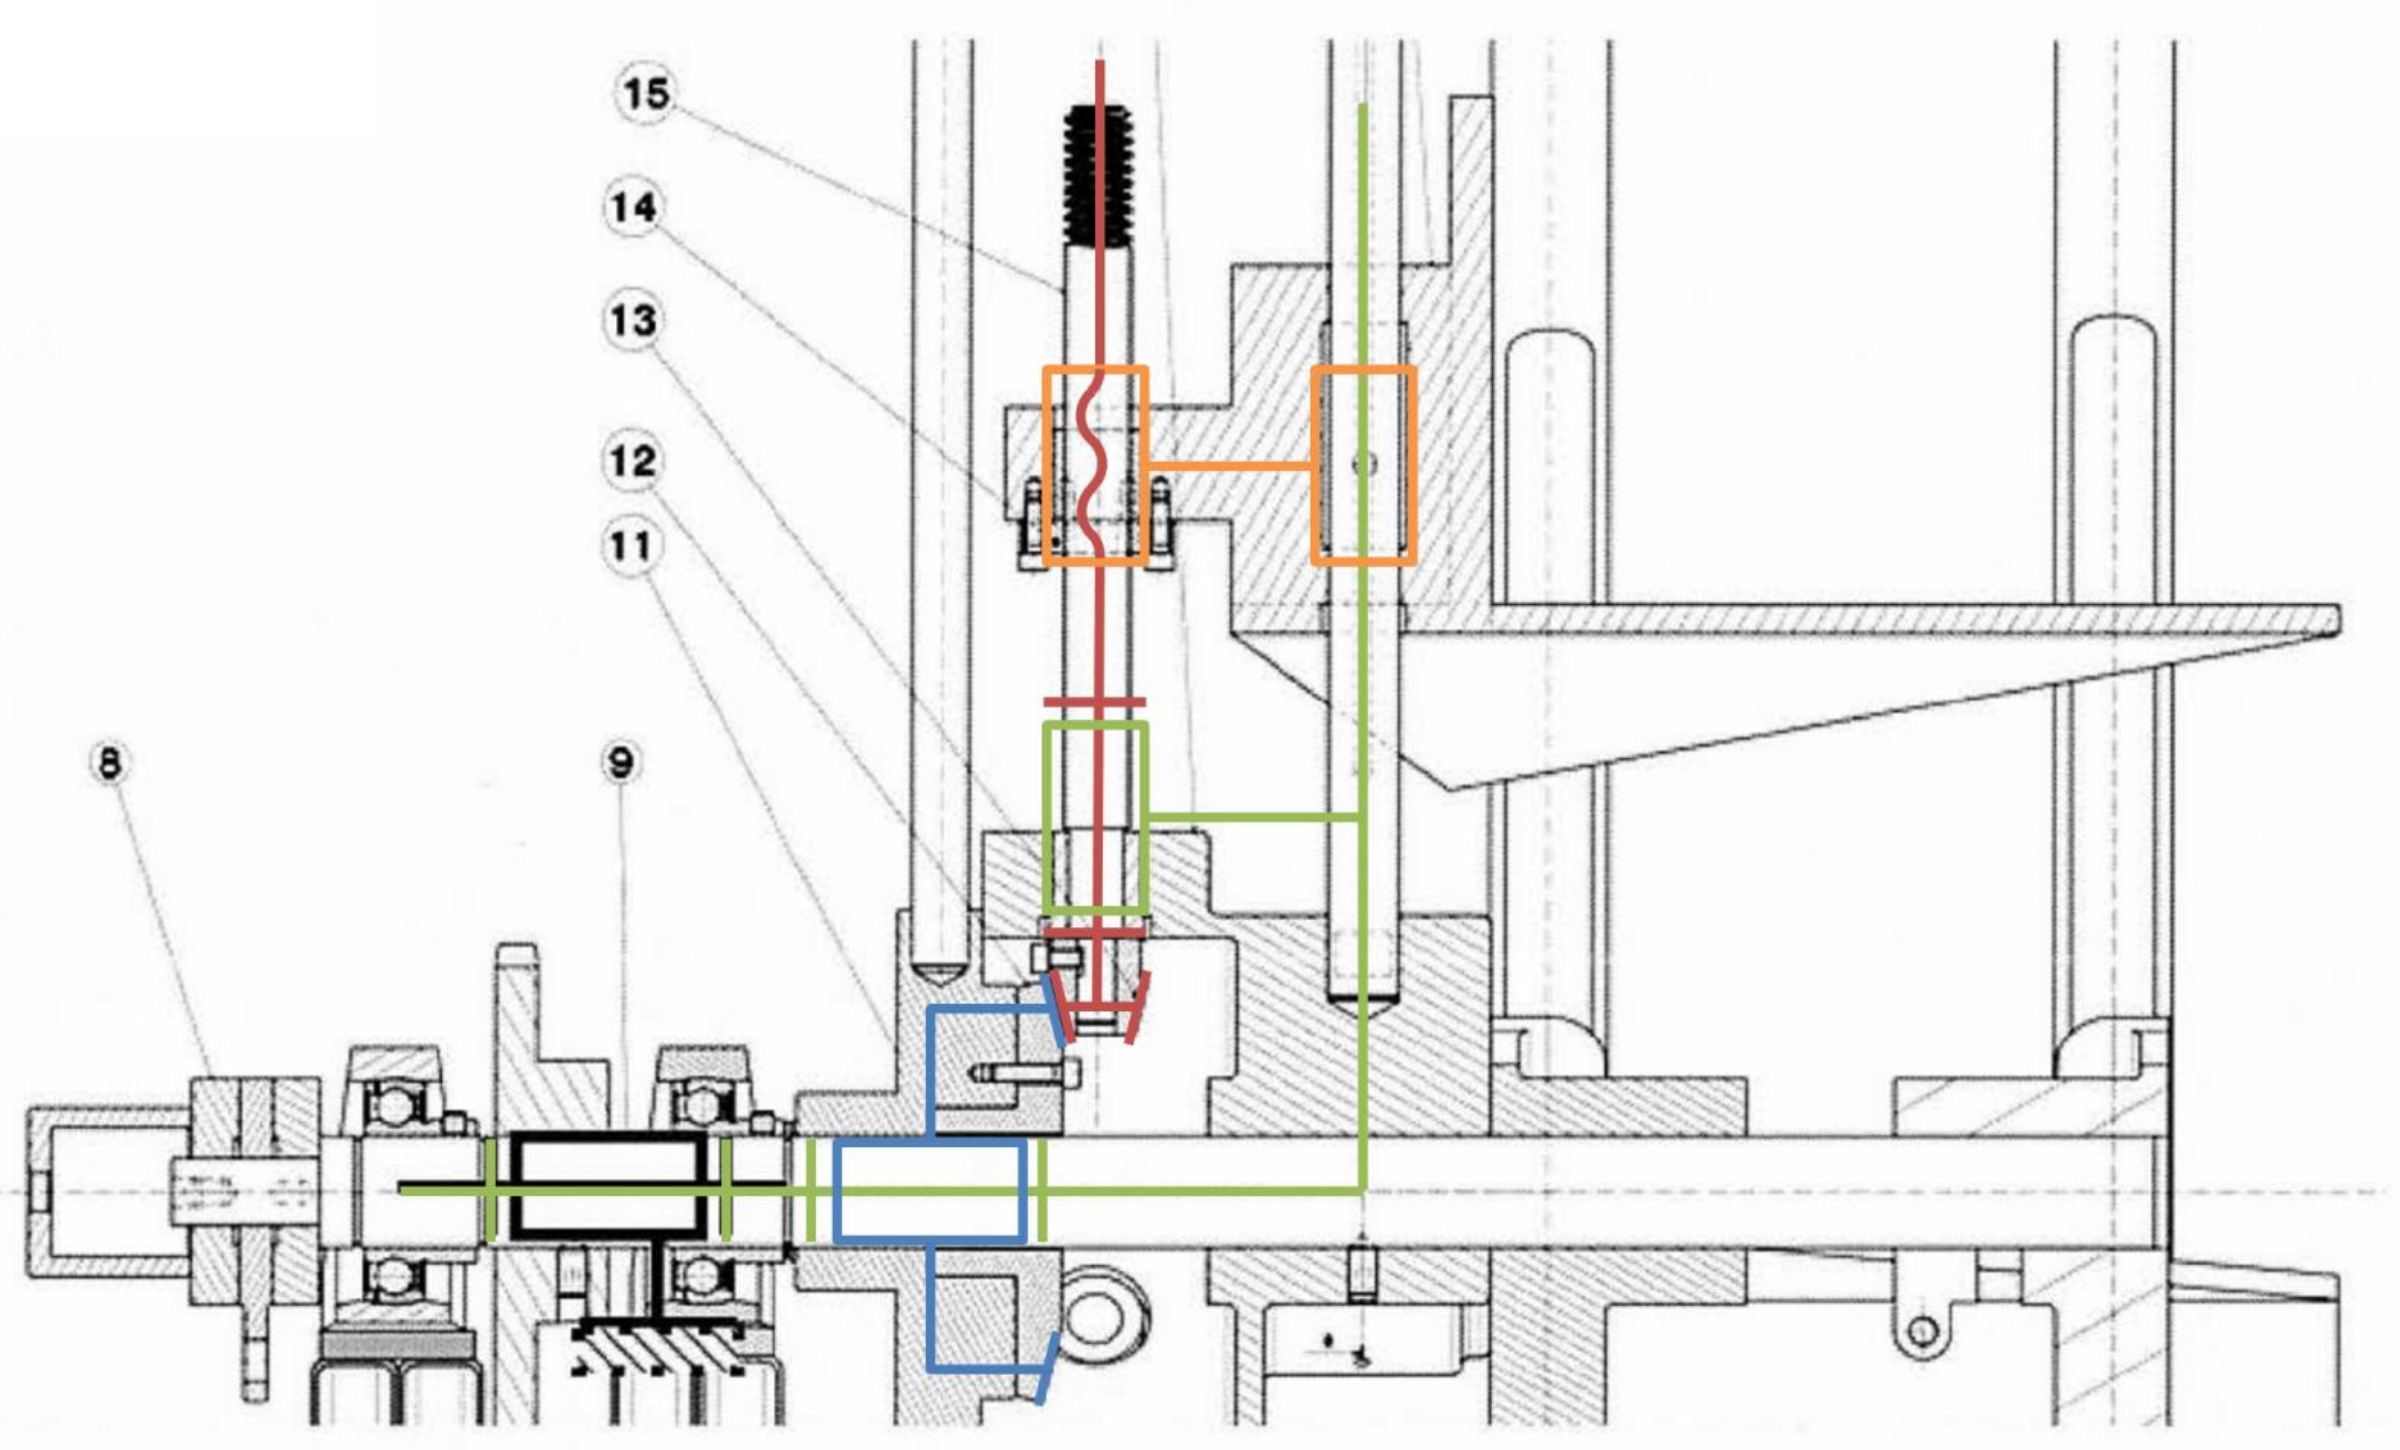
\includegraphics[width=0.9\linewidth]{img/dr20_cor}}}

\newpage

\reponse{1}{\ifdef{\public}{\vspace{-0.5cm}\begin{center}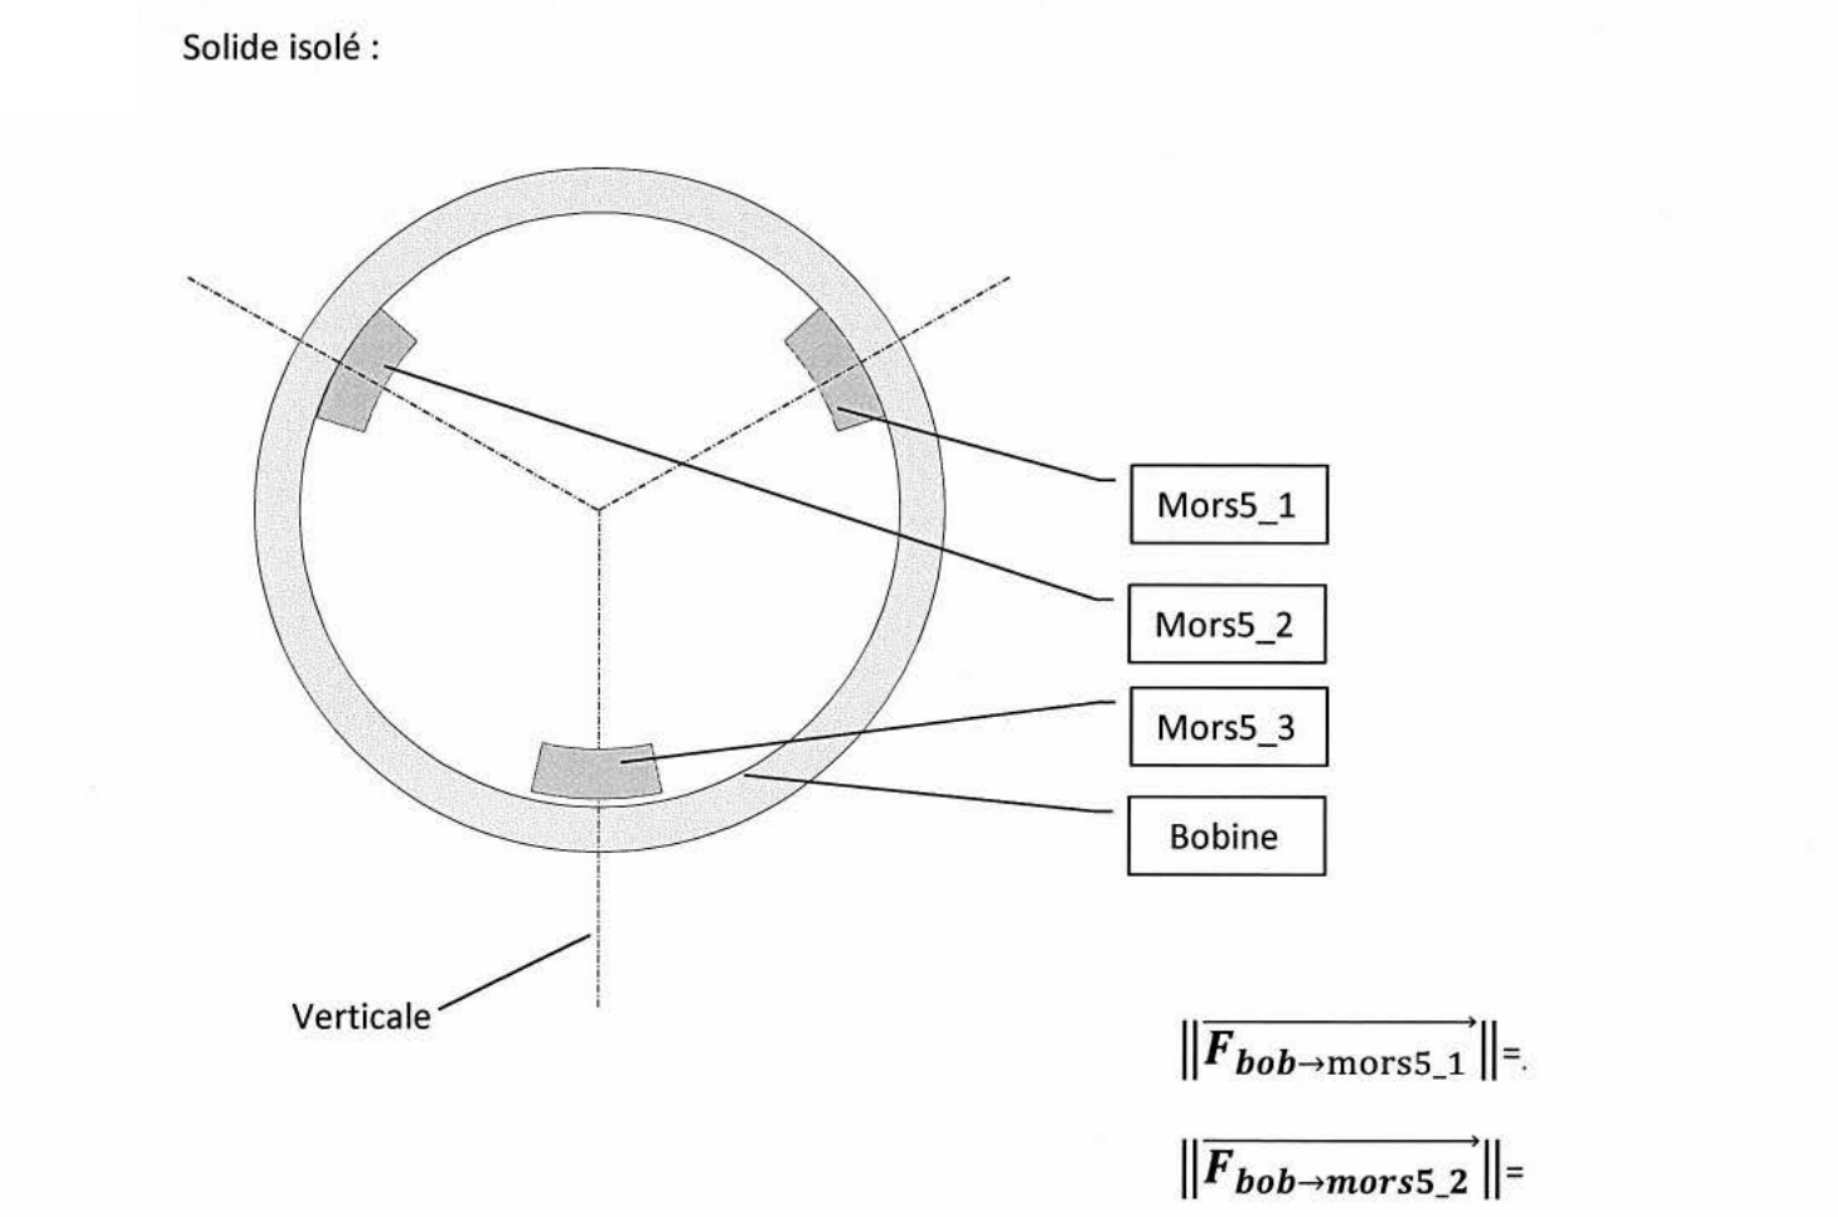
\includegraphics[width=0.8\linewidth]{img/dr21}\end{center}}{\vspace{-0.5cm}\begin{center}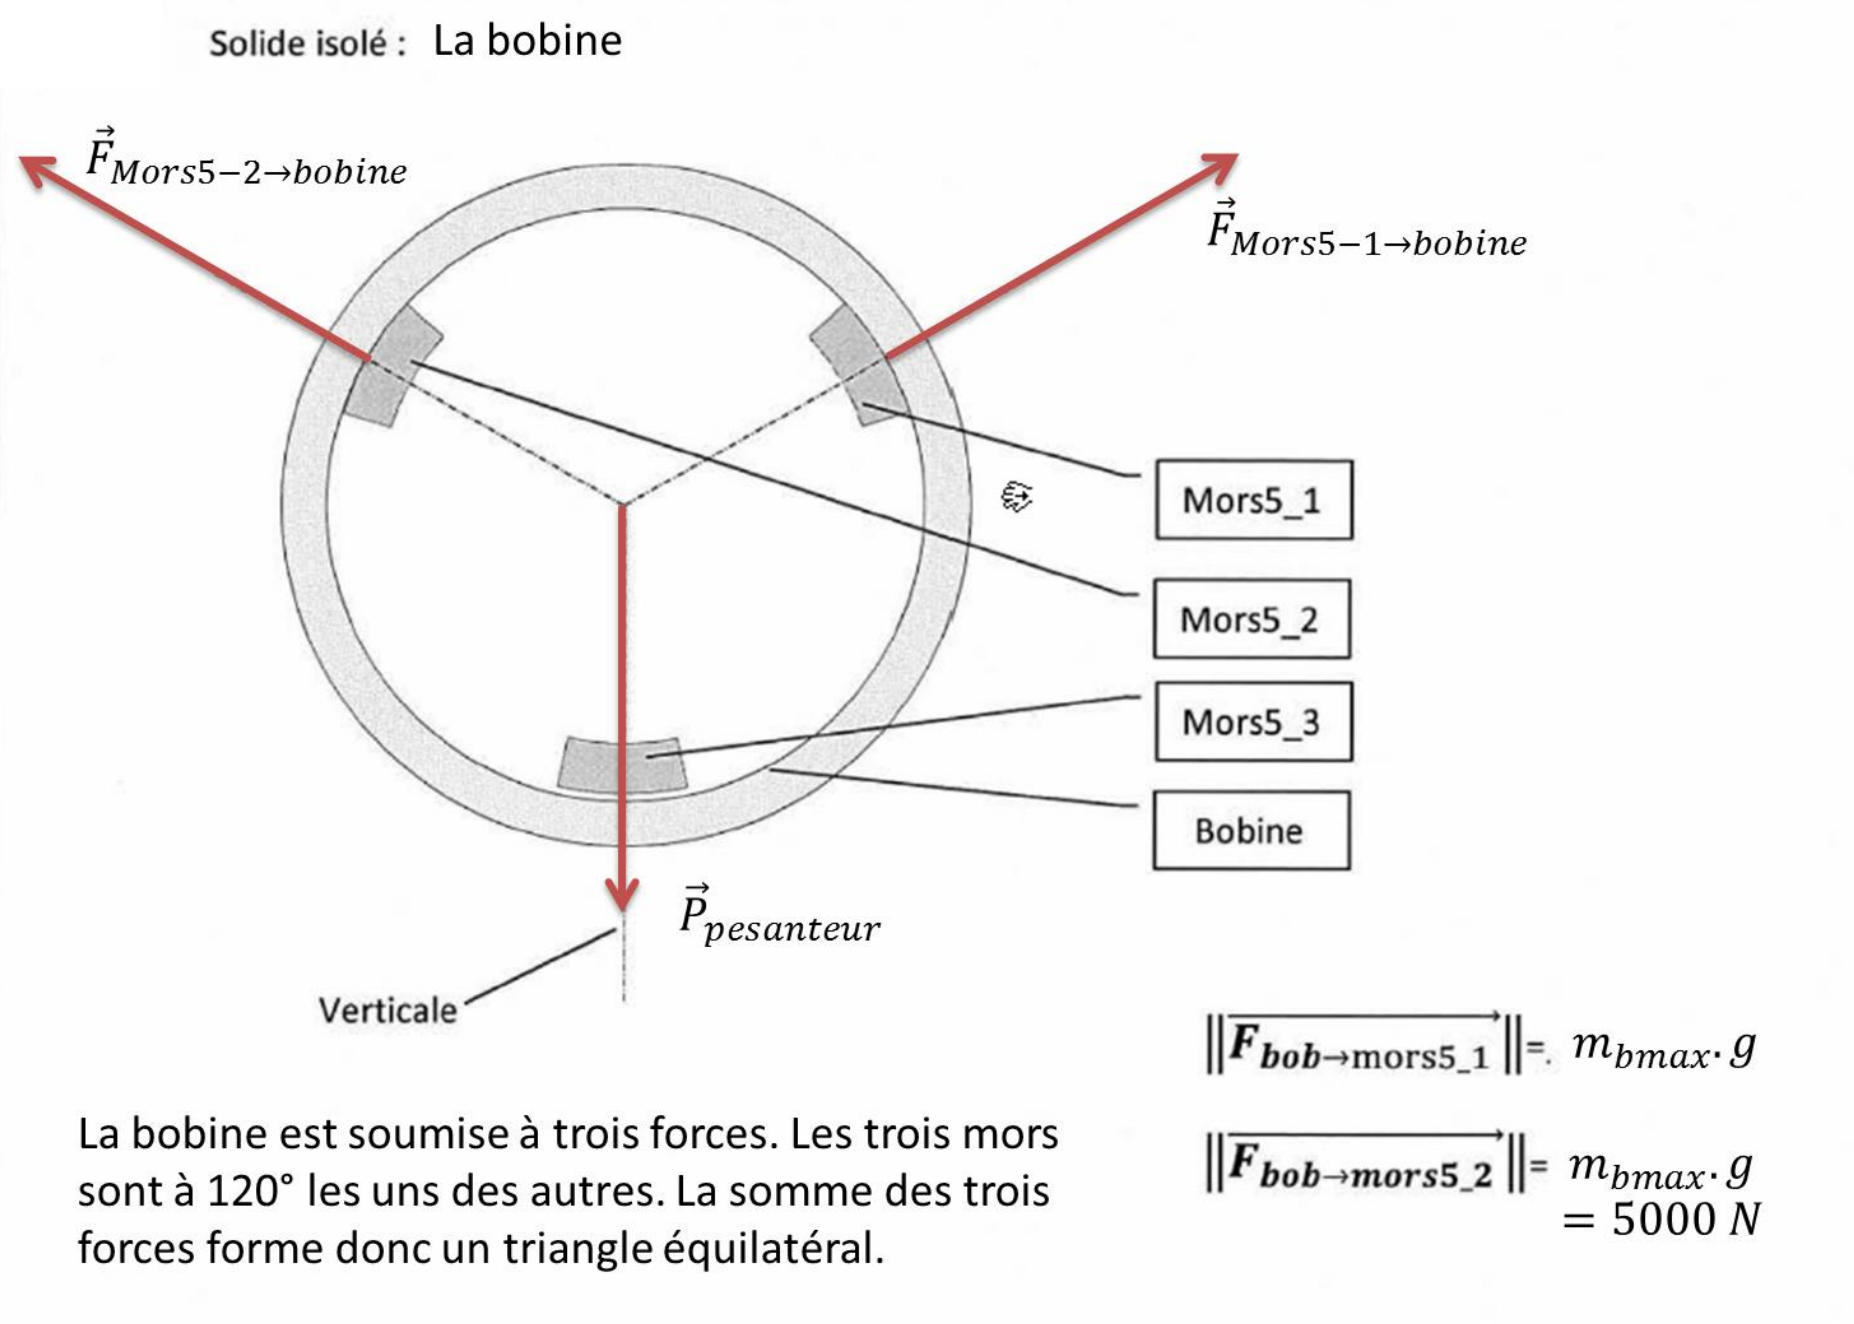
\includegraphics[width=0.7\linewidth]{img/dr21_cor}\end{center}\vspace{-0.5cm}}}

\reponse{1}{\ifdef{\public}{$\|\overrightarrow{F_{a-vis}}\|=$}{$\|\overrightarrow{F_{a-vis}}\|=Y_{VE}$}}

\reponse{1}{
Notation:
\begin{itemize}
 \item TMS/Ox signifie Théorème du Moment Statique en projection sur l'axe Ox,
 \item TRS/Oz signifie Théorème de la Résultante Statique en projection sur l'axe Oz.
\end{itemize}

~\

Cocher la (les) case(s) retenue(s):

\begin{center}
\begin{tabular}{|c|l|c|l}
\hline
& TRS/Ox & TMS/Ox \\
\hline
\ifdef{\public}{}{X}& TRS/Oy & TMS/Oy \\
\hline
& TRS/Oz & TMS/Oz \\
\hline
\end{tabular}
\end{center}}}

\reponse{1}{\ifdef{\public}{$\|\overrightarrow{F_{a-vis}}\|=$}{$\|\overrightarrow{F_{a-vis}}\|=P_{bob}$}}

\reponse{1}{\ifdef{\public}{$C_{a-vis}=$\hspace{4cm}, donc $k_1=$}{$C_{a-vis}=\frac{p_{vis}}{2.\pi.\eta_{vis}}.F_{a-vis}$, donc $k_1=\frac{p_{vis}}{2.\pi.\eta_{vis}}$}}

\reponse{1}{\ifdef{\public}{$C_{roue-unit}=$}{$C_{roue-unit}=\frac{1}{0,25}.C_{a-vis}$ \\ On suppose le rendement parfait.}}

\reponse{1}{\ifdef{\public}{$C_{ma}=$}{$C_{ma}=132N.m$. \\ 2 mors sont chargés.}}

\reponse{1}{\ifdef{\public}{$F_{op}\approx$}{$F_{op}\approx 200N.m$. Effort élevé mais réalisable.}}

\ifdef{\public}{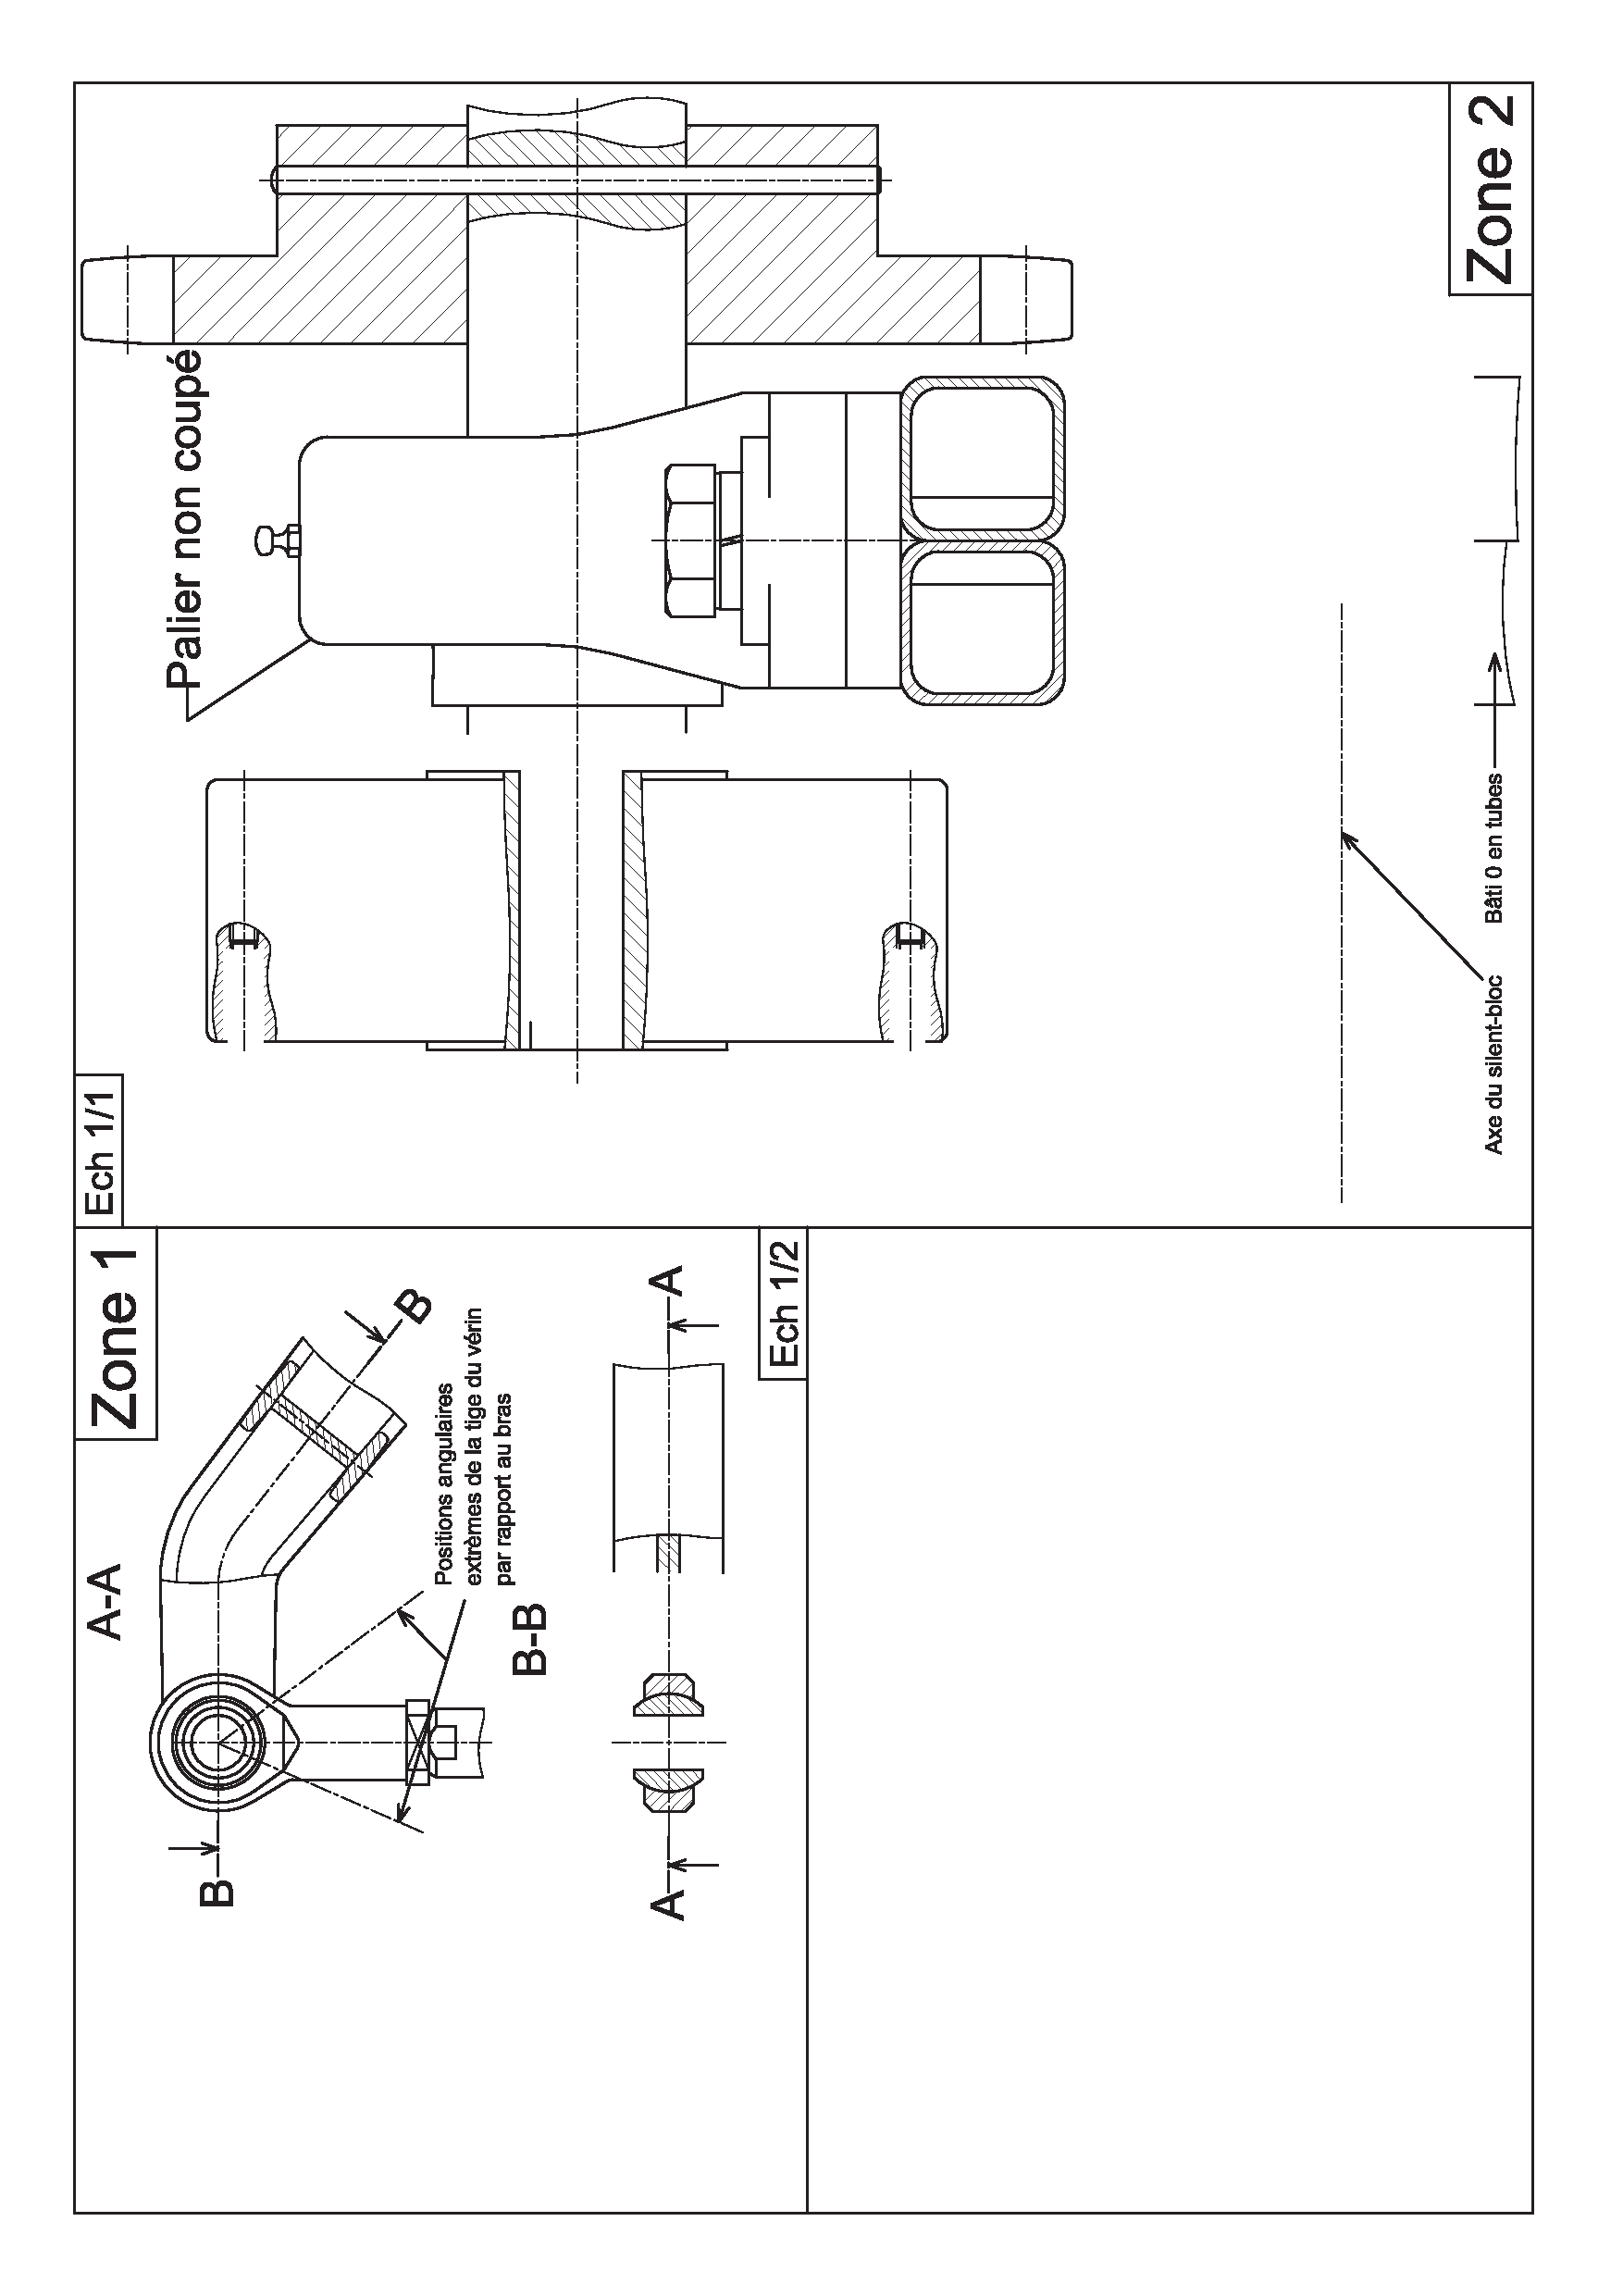
\includepdf[pages={-},templatesize={210mm}{297mm},offset=0cm -1cm]{img/calque.pdf}}{%\includepdf[pages={-},templatesize={210mm}{297mm},offset=0cm -1cm]{img/calque_c1.pdf}\includepdf[pages={-},templatesize={210mm}{297mm},offset=0cm -1cm]{img/calque_c2.pdf}
}

\end{document}
